\documentclass[11pt,a4paper]{article}

% --- Packages ---
\usepackage[utf8]{inputenc}
\usepackage[T1]{fontenc}
\usepackage{charter}
\usepackage[margin=1in]{geometry}
\usepackage{booktabs}
\usepackage{multirow}
\usepackage{graphicx}
\usepackage{amsmath,amssymb}
\usepackage[dvipsnames]{xcolor}
\usepackage[colorlinks=true,linkcolor=NavyBlue,citecolor=NavyBlue,urlcolor=NavyBlue]{hyperref}
\usepackage{natbib}
\usepackage{tikz}
\usepackage{pgfplots}
\pgfplotsset{compat=1.17}
\usetikzlibrary{patterns, calc, arrows.meta, positioning, shapes.geometric}
\usepackage{enumitem}
\usepackage{fancyhdr}
\usepackage{titlesec}
\usepackage{mdframed}
\usepackage{caption}
\usepackage{float}
\usepackage{listings}
\usepackage{tcolorbox}
\tcbuselibrary{skins,breakable}

% --- Colors ---
\definecolor{accent}{HTML}{1A3A5C}
\definecolor{lightaccent}{HTML}{E8EEF4}
\definecolor{codegreen}{HTML}{2E7D32}
\definecolor{codegray}{HTML}{757575}
\definecolor{keycolor}{HTML}{1565C0}
\definecolor{warnbg}{HTML}{FFF8E1}
\definecolor{warnborder}{HTML}{F9A825}
\definecolor{tipbg}{HTML}{E8F5E9}
\definecolor{tipborder}{HTML}{43A047}

% --- Code listings ---
\lstset{
  basicstyle=\small\ttfamily,
  keywordstyle=\color{keycolor}\bfseries,
  commentstyle=\color{codegray}\itshape,
  stringstyle=\color{codegreen},
  backgroundcolor=\color{gray!5},
  frame=single,
  rulecolor=\color{gray!30},
  breaklines=true,
  breakatwhitespace=true,
  tabsize=2,
  showstringspaces=false,
  numbers=left,
  numberstyle=\tiny\color{codegray},
  numbersep=8pt,
  xleftmargin=2em,
  framexleftmargin=1.5em,
}

% --- Custom environments ---
\newtcolorbox{keyidea}[1][]{
  colback=lightaccent,
  colframe=accent,
  fonttitle=\bfseries,
  title={Key Idea},
  #1
}

\newtcolorbox{warning}[1][]{
  colback=warnbg,
  colframe=warnborder,
  fonttitle=\bfseries,
  title={Warning},
  #1
}

\newtcolorbox{tip}[1][]{
  colback=tipbg,
  colframe=tipborder,
  fonttitle=\bfseries,
  title={Practical Tip},
  #1
}

\newtcolorbox{reporef}[1][]{
  colback=gray!5,
  colframe=gray!40,
  fonttitle=\bfseries\ttfamily,
  title={Repository Reference},
  #1
}

\newtcolorbox{buildnow}[1][]{
  colback=tipbg,
  colframe=tipborder,
  fonttitle=\bfseries,
  title={If You Are Building Now},
  #1
}

\newtcolorbox{successcheck}[1][]{
  colback=lightaccent,
  colframe=accent,
  fonttitle=\bfseries,
  title={Success Check},
  #1
}

\newtcolorbox{failuresign}[1][]{
  colback=warnbg,
  colframe=red!60!black,
  fonttitle=\bfseries,
  title={Common Failure Signs},
  #1
}

% --- Section formatting ---
\titleformat{\section}{\Large\bfseries\color{accent}}{Chapter \thesection:}{0.5em}{}[\vspace{2pt}{\color{accent}\hrule height 1.5pt}\vspace{6pt}]
\titleformat{\subsection}{\large\bfseries\color{accent}}{\thesubsection}{0.5em}{}
\titleformat{\subsubsection}{\normalsize\bfseries\color{accent!80}}{\thesubsubsection}{0.5em}{}
\titlespacing*{\section}{0pt}{24pt}{12pt}
\titlespacing*{\subsection}{0pt}{16pt}{8pt}
\titlespacing*{\subsubsection}{0pt}{12pt}{6pt}

% --- Caption styling ---
\captionsetup{font=small, labelfont=bf, textfont=it, skip=8pt}

% --- Header/Footer ---
\pagestyle{fancy}
\fancyhf{}
\fancyhead[L]{\small\color{accent}\textit{SemiticGPT: A Practical Guide to Training Multilingual Language Models}}
\fancyhead[R]{\small\color{accent}\thepage}
\renewcommand{\headrulewidth}{0.4pt}
\renewcommand{\headrule}{\hbox to\headwidth{\color{accent}\leaders\hrule height \headrulewidth\hfill}}

% --- Title ---
\title{
\vspace{-0.5in}
{\Huge\bfseries\color{accent} SemiticGPT}\\[6pt]
{\LARGE A Practical Guide to Training\\Multilingual Language Models}\\[12pt]
{\large From Theory to a Working 3-Billion Parameter Model\\for Hebrew, Arabic, Persian, and English}\\[18pt]
{\normalsize\textbf{Ronnen Slasky}}\\[4pt]
{\small Independent Researcher \quad \texttt{ronnen@gmail.com}}\\[8pt]
{\small
Code: \href{https://github.com/fatherRonnen/semitic-gpt}{\texttt{github.com/fatherRonnen/semitic-gpt}} $\cdot$
Model: \href{https://huggingface.co/Slasky/SemiticGPT-3B}{\texttt{huggingface.co/Slasky/SemiticGPT-3B}}
}\\[4pt]
{\small April 2026}
}
\author{}
\date{}

\begin{document}
\maketitle
\thispagestyle{fancy}

% ============================================================
% PREFACE
% ============================================================

\begin{tcolorbox}[colback=lightaccent, colframe=accent, title={\large\bfseries Who This Guide Is For}]
This document is for \textbf{technical people who are not AI specialists} but want to understand how language models are actually built. If you can read code, understand basic statistics, and have heard of ``GPT'' but are not sure what happens inside one, this guide is for you.

We walk through every step of building SemiticGPT---a 3.14-billion parameter language model that understands Hebrew, Arabic, Persian, and English---from the fundamental concepts to the specific code that made it work. Every section links to the actual artifacts in our \href{https://github.com/fatherRonnen/semitic-gpt}{GitHub repository}, so you can inspect, modify, and reproduce each step.

\textbf{What you will learn:}
\begin{itemize}
    \item What language models actually are and how they work
    \item The difference between model architectures and why we chose ours
    \item How to build a tokenizer for non-Latin scripts
    \item How to collect and prepare multilingual training data
    \item How to validate your approach cheaply before committing to expensive training
    \item How to train a multi-billion parameter model on cloud GPUs
    \item How to fine-tune and evaluate the result
    \item What went wrong along the way and what we learned from it
\end{itemize}

\textbf{What you will need:} Familiarity with Python, basic command-line usage, and access to cloud GPU instances (AWS, GCP, or similar). No prior machine learning experience is assumed.
\end{tcolorbox}

\vspace{12pt}

% ============================================================
% HOW TO USE THIS GUIDE
% ============================================================

\subsection*{How to Use This Guide}
\addcontentsline{toc}{subsection}{How to Use This Guide}

This guide supports two reading paths. Choose the one that matches your goal:

\begin{tcolorbox}[colback=tipbg, colframe=tipborder, fonttitle=\bfseries, title={Track A --- Learn the Concepts}]
\textbf{Goal:} Understand how multilingual language models work, from tokenization to evaluation.\\
\textbf{Time:} 3--4 hours of focused reading.\\
\textbf{Path:} Read chapters 1--5, 8--10 in order. Skim chapters 6--7 for key ideas. Use Chapter~11 as a reference.\\
\textbf{What you will get:} Deep understanding of design decisions, trade-offs, and what makes multilingual models different.
\end{tcolorbox}

\vspace{6pt}

\begin{tcolorbox}[colback=lightaccent, colframe=accent, fonttitle=\bfseries, title={Track B --- Build First}]
\textbf{Goal:} Train your own multilingual model as quickly as possible.\\
\textbf{Time:} 1--2 hours of reading, then 3--5 weeks of building.\\
\textbf{Path:} Read the ``If You Are Building Now'' boxes in chapters 3--8. Follow Chapter~11 step by step. Refer back to concept chapters when you need depth.\\
\textbf{What you will get:} A working model, with understanding built through practice.
\end{tcolorbox}

\vspace{6pt}

Every chapter is labelled with its track at the top: \textbf{Concept}, \textbf{Build}, or both. You can switch tracks at any point---the guide is designed to work either way.

\subsection*{One-Page Build Map}
\addcontentsline{toc}{subsection}{One-Page Build Map}

The entire pipeline from idea to working model:

\begin{figure}[H]
\centering
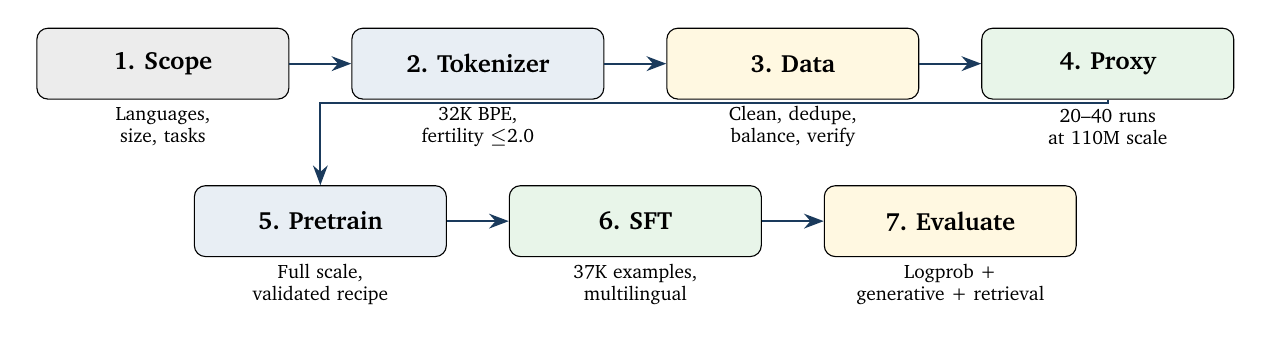
\begin{tikzpicture}[
    phase/.style={draw, rounded corners, fill=#1, minimum width=3.2cm, minimum height=0.9cm, align=center, font=\small\bfseries},
    arrow/.style={-{Stealth[length=2.5mm]}, thick, color=accent},
    note/.style={font=\scriptsize, text width=3.2cm, align=center}
]
\node[phase=gray!15] (scope) at (0, 0) {1. Scope};
\node[phase=lightaccent] (tok) at (4, 0) {2. Tokenizer};
\node[phase=warnbg] (data) at (8, 0) {3. Data};
\node[phase=tipbg] (proxy) at (12, 0) {4. Proxy};
\node[phase=lightaccent] (pretrain) at (2, -2) {5. Pretrain};
\node[phase=tipbg] (sft) at (6, -2) {6. SFT};
\node[phase=warnbg] (eval) at (10, -2) {7. Evaluate};

\node[note] at (0, -0.8) {Languages,\\size, tasks};
\node[note] at (4, -0.8) {32K BPE,\\fertility $\leq$2.0};
\node[note] at (8, -0.8) {Clean, dedupe,\\balance, verify};
\node[note] at (12, -0.8) {20--40 runs\\at 110M scale};
\node[note] at (2, -2.8) {Full scale,\\validated recipe};
\node[note] at (6, -2.8) {37K examples,\\multilingual};
\node[note] at (10, -2.8) {Logprob +\\generative + retrieval};

\draw[arrow] (scope) -- (tok);
\draw[arrow] (tok) -- (data);
\draw[arrow] (data) -- (proxy);
\draw[arrow] (proxy) -- ++(0,-0.5) -| (pretrain);
\draw[arrow] (pretrain) -- (sft);
\draw[arrow] (sft) -- (eval);
\end{tikzpicture}
\caption{The seven-phase pipeline. Chapters 1--2 provide conceptual foundations; Chapters 3--8 map to phases 2--7; Chapters 9--10 inform iteration.}
\end{figure}

\tableofcontents
\newpage

% ============================================================
% CHAPTER 1: WHAT IS A LANGUAGE MODEL?
% ============================================================

\section{What Is a Language Model?}
\label{ch:what_is_lm}

\begin{center}
\colorbox{lightaccent}{\textbf{Track: Concept + Build}}
\end{center}

\subsection{The Core Idea}

A language model is a program that predicts the next word in a sequence. That is, fundamentally, all it does. If you give it the text:

\begin{quote}
\textit{``The capital of France is \rule{2cm}{0.4pt}''}
\end{quote}

\noindent a good language model will assign a high probability to ``Paris'' and a low probability to ``banana.'' This single capability---predicting what comes next---turns out to be extraordinarily powerful. A model that is good at predicting the next word must, implicitly, understand grammar, facts, reasoning, and even style. It does not ``know'' these things the way a human does, but it has learned statistical patterns that approximate them.

\begin{keyidea}
Language models do not \emph{understand} language in the human sense. They learn statistical patterns over enormous amounts of text. But those patterns are rich enough to produce behavior that looks remarkably like understanding. The philosophical question of whether this constitutes ``real'' understanding is fascinating but outside the scope of this guide.
\end{keyidea}

\subsection{From Words to Numbers: Tokens}

Computers work with numbers, not words. Before a language model can process text, it must be converted into a sequence of numbers. This conversion happens through a \textbf{tokenizer}---a program that breaks text into smaller units called \textbf{tokens} and assigns each one a number.

Tokens are not always whole words. Depending on the tokenizer, a token might be:

\begin{itemize}
    \item A common word: ``the'' $\rightarrow$ token 1234
    \item Part of a word: ``un'' + ``believe'' + ``able'' $\rightarrow$ tokens [567, 891, 234]
    \item A single character: for rare scripts, each letter might be its own token
    \item A special marker: \texttt{<s>} (start of text) $\rightarrow$ token 1
\end{itemize}

Why not just use whole words? Because languages have enormous vocabularies. English alone has hundreds of thousands of words, and when you add Hebrew, Arabic, and Persian, the number explodes. A tokenizer that assigned one number per word would need a massive vocabulary table, and most entries would be rarely used.

Instead, modern tokenizers use \textbf{subword algorithms} (we use one called BPE, which we will explain in Chapter~\ref{ch:tokenizer}) that find a balance: common words get their own token, while rare words are broken into reusable pieces. This keeps the vocabulary manageable (our model uses 32,000 tokens) while still being able to represent any text.

\begin{tip}
The size of the vocabulary is a design choice with real consequences. Too small (say, 1,000 tokens) and every word gets chopped into many pieces, making text ``expensive'' to process. Too large (say, 1,000,000 tokens) and the model wastes capacity storing embeddings for tokens it rarely sees. For multilingual models covering 4--6 languages, 32,000--65,000 tokens is a common sweet spot.
\end{tip}

\subsection{How a Language Model Generates Text}

Once text is tokenized into numbers, the language model processes the sequence and outputs a \textbf{probability distribution} over the entire vocabulary---a list of 32,000 numbers (one per token) that says how likely each token is to come next.

For example, given ``The capital of France is'':

\begin{table}[H]
\centering
\begin{tabular}{lr}
\toprule
\textbf{Token} & \textbf{Probability} \\
\midrule
Paris & 0.85 \\
the & 0.03 \\
Lyon & 0.02 \\
a & 0.01 \\
\ldots (31,996 other tokens) & \ldots \\
banana & 0.000001 \\
\bottomrule
\end{tabular}
\caption{Simplified probability distribution. The model assigns high probability to ``Paris'' and near-zero probability to ``banana.''}
\end{table}

To generate text, we \textbf{sample} from this distribution---pick one token (usually one of the top candidates), add it to the sequence, and repeat. This is why language model output is often slightly different each time: there is randomness in the sampling step.

\begin{keyidea}
A language model produces one token at a time. To generate a paragraph, it runs hundreds of times in a loop, each time taking everything generated so far as input and predicting the next token. This is called \textbf{autoregressive generation}: the model's own output becomes part of its input for the next step.
\end{keyidea}

\subsection{What Makes This Hard for Multiple Languages?}

Building a language model for English is ``easy'' (relatively speaking) because:

\begin{enumerate}
    \item \textbf{Abundant data}: Trillions of English words are available online.
    \item \textbf{Established tokenizers}: Existing tokenizers like Llama-2's are optimized for English.
    \item \textbf{Single script}: English uses only Latin characters (A--Z).
\end{enumerate}

Our challenge is harder for several reasons:

\textbf{Multiple scripts.} Hebrew uses its own alphabet (alef-bet), Arabic uses Arabic script (which Persian also uses, but with four extra characters), and English uses Latin. These scripts have different character sets, write in different directions (Hebrew and Arabic are right-to-left), and have different rules for how letters connect.

\textbf{Rich morphology.} Hebrew and Arabic are \textbf{morphologically rich}---a single root of three consonants can generate dozens of words through patterns. The Hebrew root K-T-V (write) produces: \emph{katav} (he wrote), \emph{kotev} (he writes), \emph{miktav} (a letter), \emph{ktuva} (written), and many more. This means these languages have far more distinct word forms than English, making tokenization harder.

\textbf{Limited data.} While English has trillions of tokens available, Hebrew has perhaps tens of billions and Arabic somewhat more. Persian falls somewhere in between. This means we cannot simply throw more data at the problem---we must be efficient.

\textbf{Cross-lingual relationships.} Hebrew and Arabic are both Semitic languages---they share a common ancestor and have similar grammatical structures. Persian is unrelated (it is Indo-European, like English) but uses Arabic script and has many Arabic loanwords. We want our model to exploit these relationships: if it learns something about Hebrew grammar, can it reuse that knowledge for Arabic?

\subsection{The Two Phases of Building a Language Model}

Building a useful language model happens in two distinct phases:

\begin{enumerate}
    \item \textbf{Pretraining}: Feed the model billions of tokens of raw text. It learns language structure, facts, and cross-lingual patterns. After this phase, the model can predict text fluently but does not know how to follow instructions or perform specific tasks. Think of this as a well-read person who has never been asked a question.

    \item \textbf{Supervised Fine-Tuning (SFT)}: Show the model thousands of examples of the behavior you want---question-answer pairs, classification examples, translation pairs. This teaches the model to follow instructions and perform specific tasks. Think of this as training the well-read person to be a useful assistant.
\end{enumerate}

\begin{figure}[H]
\centering
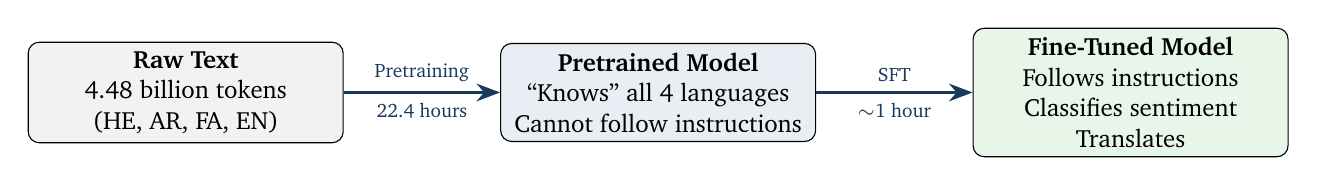
\begin{tikzpicture}[
    box/.style={draw, rounded corners, fill=#1, minimum width=4cm, minimum height=1.2cm, align=center, font=\small},
    arrow/.style={-{Stealth[length=3mm]}, thick, color=accent}
]
\node[box=gray!10] (raw) at (0,0) {\textbf{Raw Text}\\4.48 billion tokens\\(HE, AR, FA, EN)};
\node[box=lightaccent] (pretrain) at (6,0) {\textbf{Pretrained Model}\\``Knows'' all 4 languages\\Cannot follow instructions};
\node[box=tipbg] (sft) at (12,0) {\textbf{Fine-Tuned Model}\\Follows instructions\\Classifies sentiment\\Translates};

\draw[arrow] (raw) -- node[above, font=\scriptsize] {Pretraining} node[below, font=\scriptsize] {22.4 hours} (pretrain);
\draw[arrow] (pretrain) -- node[above, font=\scriptsize] {SFT} node[below, font=\scriptsize] {$\sim$1 hour} (sft);
\end{tikzpicture}
\caption{The two-phase process. Pretraining is expensive and teaches general language knowledge. Fine-tuning is cheap and teaches specific behaviors.}
\label{fig:two_phases}
\end{figure}

An important asymmetry: pretraining is computationally expensive (ours took 22.4 hours on a machine with eight high-end GPUs), while fine-tuning is cheap (about one hour on a single smaller GPU). This means you pretrain once and can fine-tune many times for different tasks.

\subsection{How Big Is 3 Billion Parameters?}

Our model has 3.14 billion \textbf{parameters}---the adjustable numbers that the model learns during training. To give some intuition:

\begin{itemize}
    \item A simple linear regression has 2 parameters (slope and intercept).
    \item A small neural network for image recognition might have 1 million parameters.
    \item GPT-2 (2019) had 1.5 billion parameters.
    \item \textbf{SemiticGPT has 3.14 billion parameters.}
    \item GPT-3 (2020) had 175 billion parameters.
    \item GPT-4 (2023) is estimated to have over 1 trillion parameters.
\end{itemize}

At 3 billion parameters, our model is small by current frontier standards but large enough to learn genuine language understanding. It cannot write essays as well as GPT-4, but it can classify sentiment, align translations, and demonstrate cross-lingual transfer---the phenomena we wanted to study.

Each parameter is stored as a \texttt{bfloat16} number (2 bytes), so the full model weighs about 6.3 GB on disk. It fits comfortably in the memory of a single modern GPU.

\subsection{What This Guide Will Build}

Over the following chapters, we will build SemiticGPT step by step:

\begin{table}[H]
\centering
\begin{tabular}{clll}
\toprule
\textbf{Ch.} & \textbf{Topic} & \textbf{Output} & \textbf{Repo Path} \\
\midrule
\ref{ch:architecture} & Architecture & Model design decisions & \texttt{pretrain/config/} \\
\ref{ch:tokenizer} & Tokenizer & 32K multilingual tokenizer & \texttt{tokenizer/} \\
\ref{ch:data} & Data & 4.48B token corpus & \texttt{data/} \\
\ref{ch:proxy} & Proxy Experiments & Validated training recipe & \texttt{proxy/} \\
\ref{ch:pretraining} & Pretraining & Base model (12.5 GB) & \texttt{pretrain/} \\
\ref{ch:sft} & Fine-Tuning & Task-capable model (6.3 GB) & \texttt{sft/} \\
\ref{ch:eval} & Evaluation & Performance measurements & \texttt{eval/} \\
\ref{ch:results} & Results & What we found & \texttt{paper/v2/} \\
\ref{ch:lessons} & Lessons & What went wrong & --- \\
\ref{ch:checklist} & Checklist & Step-by-step recipe & --- \\
\bottomrule
\end{tabular}
\caption{Guide roadmap. Each chapter produces a concrete artifact that feeds into the next.}
\label{tab:roadmap}
\end{table}

\begin{reporef}
All code referenced in this guide is available at:\\
\url{https://github.com/fatherRonnen/semitic-gpt}\\[4pt]
Model weights are available at:\\
\url{https://huggingface.co/Slasky/SemiticGPT-3B}
\end{reporef}

% ============================================================
% CHAPTER 2: PLACEHOLDER
% ============================================================

\section{Choosing an Architecture: Encoders, Decoders, and Why It Matters}
\label{ch:architecture}

\begin{center}
\colorbox{lightaccent}{\textbf{Track: Concept}}
\end{center}

\begin{tip}[title={For Build-First Readers}]
This chapter covers architecture theory. If you are following Track~B (build first), treat this as a reference. Skip to Chapter~3 (Tokenizer) for your first hands-on step. Come back here when you want to understand \emph{why} the architecture works.
\end{tip}

Before you can train a language model, you must choose its architecture---the blueprint that determines how information flows through the model. This choice affects what your model can do, how it is trained, and how it is used. The dominant architecture in modern NLP is the \textbf{transformer} \citep{vaswani2017attention}, but there are three major variants, and they are suited to different tasks.

\subsection{The Transformer: A Brief History}

Before 2017, most language models used architectures called \textbf{recurrent neural networks (RNNs)} that processed text one word at a time, left to right. This was slow (you could not parallelize it) and caused problems with long sequences (by the time the model reached word 500, it had largely ``forgotten'' word 1).

The transformer, introduced by \citet{vaswani2017attention}, solved both problems with a mechanism called \textbf{attention}: instead of reading text sequentially, the model looks at all words simultaneously and learns which words are relevant to which other words. This is massively parallelizable on GPUs and handles long-range dependencies naturally.

\begin{keyidea}
The key insight of the transformer is \textbf{attention}: for each word in the input, the model computes a weighted combination of all other words, where the weights reflect relevance. ``The cat sat on the mat because \emph{it} was tired''---to understand ``it,'' the model attends strongly to ``cat'' and weakly to ``mat,'' even though ``mat'' is closer.
\end{keyidea}

The original transformer had two halves: an \textbf{encoder} (which reads the input) and a \textbf{decoder} (which generates the output). Subsequent research found that you could use just one half and still get excellent results, leading to three families:

\subsection{The Three Families}

\subsubsection{Encoder-Only Models (BERT family)}

\textbf{How they work:} The model reads the \emph{entire} input at once, in both directions. Every word can attend to every other word, including words that come \emph{after} it. This is called \textbf{bidirectional} attention.

\textbf{Training method:} Mask out random words and ask the model to predict them. For example:

\begin{quote}
\texttt{The [MASK] sat on the mat} $\rightarrow$ predict ``cat''
\end{quote}

This is called \textbf{masked language modeling (MLM)}. The model learns by filling in blanks, which forces it to understand context from both sides.

\textbf{What they are good at:}
\begin{itemize}
    \item \textbf{Classification}: Is this review positive or negative? What language is this?
    \item \textbf{Named entity recognition}: Which words are person names, locations, organizations?
    \item \textbf{Semantic similarity}: Are these two sentences saying the same thing?
    \item \textbf{Information retrieval}: Find the most relevant document for this query.
\end{itemize}

\textbf{What they cannot do:} Generate text. Because they see the whole input at once, they have no mechanism for producing text one token at a time. You cannot ask BERT to write a paragraph.

\textbf{Famous examples:} BERT \citep{devlin2019bert}, RoBERTa, XLM-R \citep{conneau2020unsupervised}, mBERT.

\begin{figure}[H]
\centering
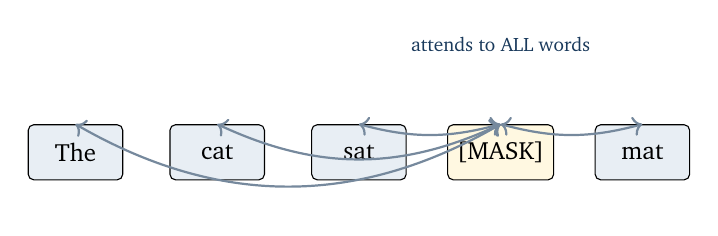
\begin{tikzpicture}[
    token/.style={draw, rounded corners=2pt, minimum width=1.2cm, minimum height=0.7cm, font=\small},
    attn/.style={<->, thick, color=accent!60}
]
\node[token, fill=lightaccent] (t1) at (0,0) {The};
\node[token, fill=lightaccent] (t2) at (1.8,0) {cat};
\node[token, fill=lightaccent] (t3) at (3.6,0) {sat};
\node[token, fill=warnbg] (t4) at (5.4,0) {[MASK]};
\node[token, fill=lightaccent] (t5) at (7.2,0) {mat};

\draw[attn] (t4.north) to[bend left=30] (t1.north);
\draw[attn] (t4.north) to[bend left=25] (t2.north);
\draw[attn] (t4.north) to[bend left=15] (t3.north);
\draw[attn] (t4.north) to[bend right=15] (t5.north);

\node[font=\scriptsize\color{accent}, above=0.8cm of t4] {attends to ALL words};
\end{tikzpicture}
\caption{Encoder-only (BERT-style): The masked token attends to all other tokens, both left and right. This bidirectional context makes encoders excellent at understanding but unable to generate.}
\label{fig:encoder}
\end{figure}

\subsubsection{Decoder-Only Models (GPT family)}

\textbf{How they work:} The model reads text left to right. Each word can only attend to words that came \emph{before} it (and itself). It never ``peeks ahead.'' This is called \textbf{causal} or \textbf{autoregressive} attention.

\textbf{Training method:} Predict the next token. Given ``The cat sat,'' predict ``on.'' Given ``The cat sat on,'' predict ``the.'' This is called \textbf{causal language modeling (CLM)}. The model processes the entire sequence in one pass, but each position can only see preceding positions.

\textbf{What they are good at:}
\begin{itemize}
    \item \textbf{Text generation}: Write articles, code, poetry, translations.
    \item \textbf{Chat and instruction following}: Answer questions, follow complex prompts.
    \item \textbf{Few-shot learning}: Give a few examples in the prompt and the model generalizes.
    \item \textbf{Classification} (with a trick): Frame it as text generation---``Is this positive or negative? Answer:'' and check what the model generates.
\end{itemize}

\textbf{What they are less good at:} Pure classification tasks where bidirectional context would help. However, in practice, large enough decoder models can match or beat encoder models even on classification by using the generation trick described above.

\textbf{Famous examples:} GPT \citep{radford2018gpt}, GPT-2 \citep{radford2019gpt2}, GPT-3 \citep{brown2020gpt3}, GPT-4, Llama, Mistral, \textbf{SemiticGPT (this project)}.

\begin{figure}[H]
\centering
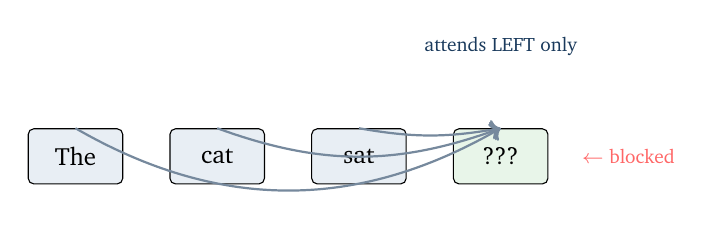
\begin{tikzpicture}[
    token/.style={draw, rounded corners=2pt, minimum width=1.2cm, minimum height=0.7cm, font=\small},
    attn/.style={<-, thick, color=accent!60},
    noattn/.style={<-, thick, color=red!30, dashed}
]
\node[token, fill=lightaccent] (t1) at (0,0) {The};
\node[token, fill=lightaccent] (t2) at (1.8,0) {cat};
\node[token, fill=lightaccent] (t3) at (3.6,0) {sat};
\node[token, fill=tipbg] (t4) at (5.4,0) {???};

\draw[attn] (t4.north) to[bend left=30] (t1.north);
\draw[attn] (t4.north) to[bend left=20] (t2.north);
\draw[attn] (t4.north) to[bend left=10] (t3.north);

\node[font=\scriptsize\color{accent}, above=0.8cm of t4] {attends LEFT only};
\node[font=\scriptsize\color{red!60}, right=0.3cm of t4] {$\leftarrow$ blocked};
\end{tikzpicture}
\caption{Decoder-only (GPT-style): Each position attends only to previous positions. This constraint enables generation: the model never sees future tokens, so it can produce them one by one.}
\label{fig:decoder}
\end{figure}

\subsubsection{Encoder-Decoder Models (T5 family)}

\textbf{How they work:} Two separate transformer stacks. The encoder reads the full input bidirectionally (like BERT). The decoder generates output autoregressively (like GPT), but can also attend to the encoder's representations. This is the original transformer architecture.

\textbf{Training method:} Varies, but T5 \citep{raffel2020t5} uses a \textbf{span corruption} objective: mask out random spans of text and ask the model to generate just the missing pieces.

\textbf{What they are good at:}
\begin{itemize}
    \item \textbf{Translation}: Read source language (encoder), generate target language (decoder).
    \item \textbf{Summarization}: Read long document (encoder), generate summary (decoder).
    \item \textbf{Structured output}: Any task that maps one text to another.
\end{itemize}

\textbf{Trade-off:} More complex, harder to scale, and the encoder and decoder must be sized relative to each other. In practice, decoder-only models have won the scaling race because they are simpler and more flexible.

\textbf{Famous examples:} T5 \citep{raffel2020t5}, mT5, BART, mBART.

\subsection{Side-by-Side Comparison}

\begin{table}[H]
\centering\small
\begin{tabular}{lccc}
\toprule
\textbf{Property} & \textbf{Encoder} & \textbf{Decoder} & \textbf{Enc-Dec} \\
 & (BERT) & (GPT) & (T5) \\
\midrule
Attention direction & Bidirectional & Left-only & Both \\
Can generate text? & No & \textbf{Yes} & \textbf{Yes} \\
Can classify? & \textbf{Yes} & Yes (trick) & Yes \\
Training objective & Fill blanks & Predict next & Fill spans \\
Scaling simplicity & Medium & \textbf{Simple} & Complex \\
Parameter efficiency & High & Medium & Lower \\
Dominant use today & Embeddings & \textbf{Chat, gen.} & Translation \\
\bottomrule
\end{tabular}
\caption{Comparison of the three transformer families. Decoder-only models dominate current large-scale development due to their simplicity and flexibility.}
\label{tab:arch_comparison}
\end{table}

\subsection{Why We Chose Decoder-Only}

For SemiticGPT, we chose the decoder-only architecture. Here is why:

\begin{enumerate}
    \item \textbf{Flexibility.} A decoder-only model can generate text \emph{and} classify. An encoder-only model can only classify. Since we wanted to study both generation and classification across languages, the decoder gives us more options with one model.

    \item \textbf{Simplicity.} Decoder-only models have one transformer stack, one training objective (predict the next token), and one inference mode. This means fewer hyperparameters to tune, simpler code, and fewer things that can go wrong. When you are training a model from scratch on a budget, simplicity matters.

    \item \textbf{Ecosystem.} The open-source ecosystem in 2025--2026 is overwhelmingly decoder-only. Llama, Mistral, SmolLM3 \citep{allal2025smollm3}---the models with the best training recipes, the most community support, and the most tooling are all GPT-style decoders. Swimming with the current means we can reuse proven techniques.

    \item \textbf{Cross-lingual transfer research.} We specifically wanted to test whether a decoder model develops cross-lingual representations during pretraining. Encoder models like XLM-R \citep{conneau2020unsupervised} are already known to do this well. Whether \emph{decoder} models do it at small scale was an open question.

    \item \textbf{SFT compatibility.} The entire instruction-tuning and chat paradigm is built around decoder models. If you want your model to follow instructions (``Classify this as positive or negative''), decoder-only is the natural fit.
\end{enumerate}

\begin{warning}
Choosing decoder-only means accepting a trade-off: for \emph{pure} classification tasks (no generation needed), an encoder model of the same size will usually be more accurate. If your only goal is building a sentiment classifier, fine-tuning XLM-R would be more efficient. We chose the decoder because our goals were broader.
\end{warning}

\subsection{Inside the Decoder: Building Blocks}

Now that we have chosen the decoder-only architecture, let us look at what is inside. A decoder is a stack of identical \textbf{layers} (we use 26), each containing the same three components:

\begin{figure}[H]
\centering
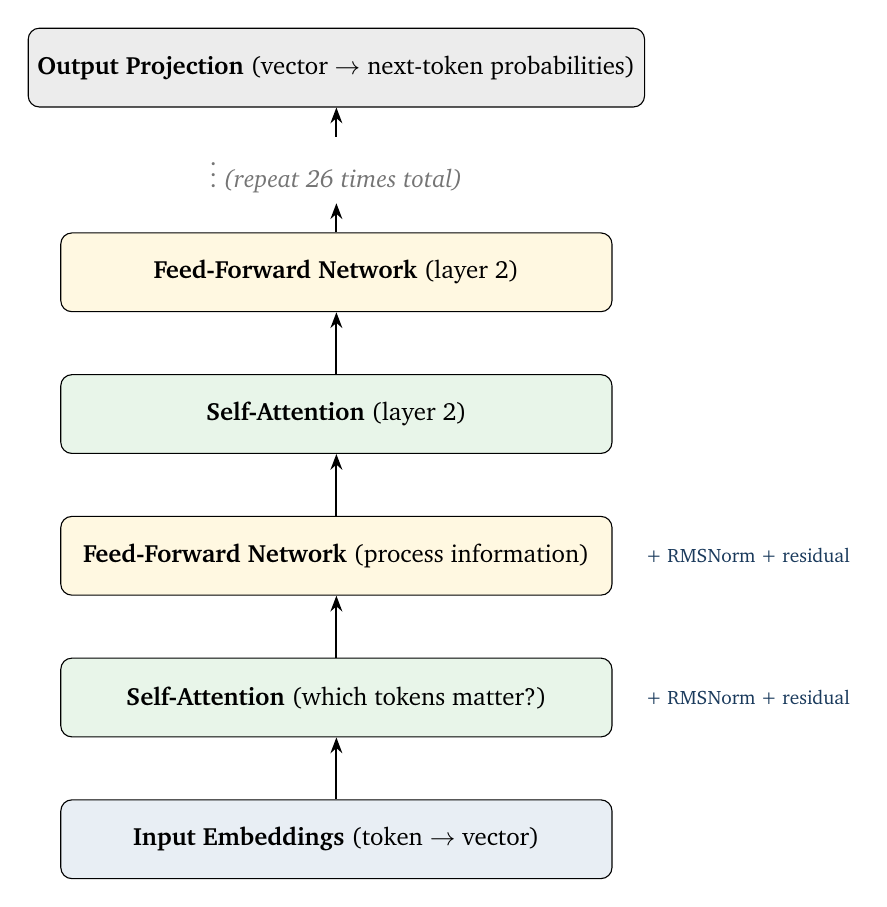
\begin{tikzpicture}[
    block/.style={draw, rounded corners, fill=#1, minimum width=7cm, minimum height=1cm, align=center, font=\small},
    arrow/.style={-{Stealth[length=2mm]}, thick}
]
\node[block=lightaccent] (input) at (0, 0) {\textbf{Input Embeddings} (token $\rightarrow$ vector)};
\node[block=tipbg] (attn) at (0, 1.8) {\textbf{Self-Attention} (which tokens matter?)};
\node[block=warnbg] (ffn) at (0, 3.6) {\textbf{Feed-Forward Network} (process information)};
\node[block=tipbg] (attn2) at (0, 5.4) {\textbf{Self-Attention} (layer 2)};
\node[block=warnbg] (ffn2) at (0, 7.2) {\textbf{Feed-Forward Network} (layer 2)};
\node[font=\small, color=codegray] (dots) at (0, 8.5) {$\vdots$ \textit{(repeat 26 times total)}};
\node[block=gray!15] (output) at (0, 9.8) {\textbf{Output Projection} (vector $\rightarrow$ next-token probabilities)};

\draw[arrow] (input) -- (attn);
\draw[arrow] (attn) -- (ffn);
\draw[arrow] (ffn) -- (attn2);
\draw[arrow] (attn2) -- (ffn2);
\draw[arrow] (ffn2) -- (dots);
\draw[arrow] (dots) -- (output);

\node[font=\scriptsize\color{accent}, right=0.3cm of attn] {+ RMSNorm + residual};
\node[font=\scriptsize\color{accent}, right=0.3cm of ffn] {+ RMSNorm + residual};
\end{tikzpicture}
\caption{SemiticGPT's architecture: 26 identical layers, each with self-attention and a feed-forward network, plus normalization and residual connections. Input tokens are converted to vectors; the final layer converts vectors back to token probabilities.}
\label{fig:architecture}
\end{figure}

\subsubsection{Self-Attention: Which Words Matter?}

Self-attention is the mechanism that lets each token ``look at'' other tokens in the sequence and decide how much to pay attention to each one. Here is the intuition:

Consider the sentence: ``The bank by the river was flooded.'' To understand ``bank,'' the model must attend to ``river'' and ``flooded'' (which tell it this is a riverbank, not a financial bank). Self-attention learns these relevance patterns automatically from data.

Mechanically, each token is transformed into three vectors:
\begin{itemize}
    \item \textbf{Query (Q)}: ``What am I looking for?''
    \item \textbf{Key (K)}: ``What do I contain?''
    \item \textbf{Value (V)}: ``What information do I provide?''
\end{itemize}

The attention score between two tokens is the dot product of one token's Query with the other's Key. High scores mean high relevance, and the output is a weighted sum of all Values.

SemiticGPT uses \textbf{24 attention heads}---24 independent sets of Q/K/V, each with a head dimension of 128. Different heads can learn different types of relationships (one might learn syntactic structure, another might learn semantic similarity). Their outputs are concatenated: $24 \times 128 = 3072$, which equals our hidden dimension.

\begin{keyidea}
The \textbf{causal mask} is what makes a decoder a decoder. During attention, we add a mask that sets all attention scores to $-\infty$ for future positions. This means token 5 can attend to tokens 1--5 but not tokens 6, 7, 8, etc. This constraint is what enables autoregressive generation.
\end{keyidea}

\subsubsection{Positional Encoding: RoPE}

Attention is \textbf{permutation-invariant}---without positional information, the model cannot tell the difference between ``dog bites man'' and ``man bites dog.'' We need a way to encode \emph{where} each token is in the sequence.

SemiticGPT uses \textbf{Rotary Position Embedding (RoPE)} \citep{su2021rope}, which encodes position by rotating the Query and Key vectors by an angle proportional to their position. Tokens that are close together have similar rotations, which naturally biases attention toward nearby tokens while still allowing long-range attention.

RoPE has two practical advantages over older methods: it handles sequences of any length (up to our maximum of 2,048 tokens), and it encodes \emph{relative} position (how far apart two tokens are) rather than absolute position, which generalizes better.

\subsubsection{Feed-Forward Network: SwiGLU}

After attention determines \emph{which} information is relevant, the feed-forward network (FFN) \emph{processes} that information. Each layer's FFN is a small two-layer neural network that operates on each token independently.

SemiticGPT uses \textbf{SwiGLU} \citep{shazeer2020glu}, a modern activation function that combines a smooth gating mechanism with a nonlinear transformation. The practical effect: better training stability and slightly better final performance compared to the older ReLU activation, at the cost of about 50\% more parameters in the FFN layer.

\subsubsection{Normalization: RMSNorm}

Deep networks are unstable---values can grow exponentially large or vanish to zero as they pass through many layers. \textbf{Normalization} keeps values in a reasonable range after each sub-layer.

SemiticGPT uses \textbf{RMSNorm} (Root Mean Square Normalization) \citep{zhang2019rms}, applied \emph{before} each attention and FFN block (called ``pre-norm''). RMSNorm is simpler and faster than the more common LayerNorm, and works equally well in practice. It normalizes by dividing by the root-mean-square of the values, with a learned scaling parameter.

\subsubsection{Residual Connections}

Each sub-layer (attention and FFN) has a \textbf{residual connection}: the sub-layer's input is \emph{added} to its output. So if the input is $x$ and the sub-layer computes $f(x)$, the output is $x + f(x)$.

This simple trick is essential for training deep networks. It creates a ``highway'' for gradients to flow backward through many layers during training, preventing the vanishing gradient problem. Without residual connections, training a 26-layer network would be very difficult.

\subsection{SemiticGPT's Specific Configuration}

\begin{table}[H]
\centering
\begin{tabular}{llp{7cm}}
\toprule
\textbf{Parameter} & \textbf{Value} & \textbf{Why this choice} \\
\midrule
Parameters & 3.14B & Large enough for meaningful language understanding; small enough to train on one node and fit on one GPU for inference. \\
Layers & 26 & Standard depth for 3B-class models. More layers = more capacity for abstract reasoning. \\
Hidden dim & 3,072 & Determines the ``width'' of information flowing through the model. 24 heads $\times$ 128 dim = 3,072. \\
Attention heads & 24 & Each head can specialize in different types of relationships. 24 is standard for this model size. \\
Head dimension & 128 & The size of each attention head. 128 is the modern default (older models used 64). \\
Vocab size & 32,000 & Balances coverage of 4 languages against embedding table size. See Chapter~\ref{ch:tokenizer}. \\
Max sequence & 2,048 & How much text the model can process at once. Sufficient for most tasks; longer sequences cost quadratically more memory. \\
Position encoding & RoPE & Handles variable-length sequences and relative positions naturally. \\
Activation & SwiGLU & Better than ReLU for training stability. Standard in modern models. \\
Normalization & RMSNorm & Simpler and faster than LayerNorm. Applied before each sub-layer (pre-norm). \\
\bottomrule
\end{tabular}
\caption{SemiticGPT architecture choices and rationale. See \texttt{pretrain/config/training\_config.json} in the repository.}
\label{tab:arch_choices}
\end{table}

\begin{reporef}
\textbf{Architecture configuration:}\hfill\texttt{pretrain/config/training\_config.json}\\
\textbf{Model implementation:}\hfill\texttt{pretrain/scripts/train\_multilingual\_3b\_fsdp.py}\\

The model definition starts around line 60 of the FSDP training script. The architecture is defined in pure PyTorch---no framework dependencies. Key classes: \texttt{Block} (one transformer layer), \texttt{GPT} (the full model with all layers, embeddings, and output projection).
\end{reporef}

\subsection{How Parameters Add Up}

Where do 3.14 billion parameters come from? Here is a rough breakdown:

\begin{table}[H]
\centering\small
\begin{tabular}{lrr}
\toprule
\textbf{Component} & \textbf{Parameters} & \textbf{\% of Total} \\
\midrule
Token embeddings ($32{,}000 \times 3{,}072$) & 98M & 3.1\% \\
Attention QKV projections ($26 \times 3 \times 3{,}072 \times 3{,}072$) & 738M & 23.5\% \\
Attention output projections ($26 \times 3{,}072 \times 3{,}072$) & 246M & 7.8\% \\
FFN (SwiGLU, 3 matrices per layer) & 1,769M & 56.3\% \\
RMSNorm parameters ($26 \times 2 + 1$ layers) & $<$1M & $<$0.1\% \\
Output projection (tied with embeddings) & 0 & 0\% \\
\midrule
\textbf{Total} & $\sim$\textbf{3,140M} & \textbf{100\%} \\
\bottomrule
\end{tabular}
\caption{Parameter breakdown. The feed-forward networks account for over half of all parameters, which is typical for transformer models. The attention mechanism accounts for about a third.}
\label{tab:param_breakdown}
\end{table}

\begin{tip}
Notice that the token embeddings (the table mapping token IDs to vectors) are \textbf{shared} with the output projection (the table mapping vectors back to token probabilities). This is called \textbf{weight tying} and saves 98M parameters with no quality loss---the intuition is that the ``meaning'' of a token should be the same whether the model is reading it or producing it.
\end{tip}

\subsection{Summary: What You Need to Decide}

If you are building your own language model, the architecture decisions boil down to:

\begin{enumerate}
    \item \textbf{Encoder, decoder, or encoder-decoder?} For most modern use cases involving generation or instruction-following, decoder-only is the default choice.
    \item \textbf{How many parameters?} Constrained by your GPU budget. Aim for the largest model you can afford to train to completion---an undertrained large model is worse than a well-trained smaller one.
    \item \textbf{Depth vs.\ width?} For a given parameter budget, modern practice favors deeper (more layers) over wider (larger hidden dimension), but the difference is small.
    \item \textbf{Vocabulary size?} 32K--64K for multilingual models. See Chapter~\ref{ch:tokenizer}.
    \item \textbf{Everything else:} Use the modern defaults (RoPE, SwiGLU, RMSNorm, pre-norm) unless you have a specific reason not to. These choices are battle-tested and well-supported in existing code.
\end{enumerate}

% ============================================================
% CHAPTER 3: PLACEHOLDER
% ============================================================

\section{Building a Multilingual Tokenizer}
\label{ch:tokenizer}

\begin{center}
\colorbox{lightaccent}{\textbf{Track: Concept + Build}}
\end{center}

Before a language model can process any text, that text must be converted into numbers. The component that does this is the \textbf{tokenizer}, and for a multilingual model, it is one of the most consequential design decisions you will make. A bad tokenizer can cripple your model before training even begins.

\begin{buildnow}
\textbf{Outcome:} A trained SentencePiece BPE tokenizer with 32K vocabulary that handles all your target languages efficiently.

\textbf{Decisions required:}
\begin{itemize}[nosep]
  \item Vocabulary size (32K or 64K)
  \item Language balance in tokenizer training data
  \item Special tokens for your downstream tasks
\end{itemize}

\textbf{Safe defaults:} 32K vocabulary, equal language proportions, SentencePiece BPE with byte fallback and NFKC normalization.

\textbf{Skip on first pass:} The specialization trade-off analysis (\S\ref{ch:tokenizer}.7). Come back after you see fertility results.
\end{buildnow}

\subsection{Why Tokenization Matters}

Consider a simple thought experiment. Suppose your tokenizer was designed for English and you feed it a Hebrew sentence. The tokenizer has never seen Hebrew characters, so it falls back to encoding each character---or even each \emph{byte}---as a separate token. A five-word Hebrew sentence might become 40 tokens, while the equivalent English sentence might be 7 tokens.

This has three consequences:

\begin{enumerate}
    \item \textbf{Wasted context window.} If your model can process 2,048 tokens at a time, the English user gets $\sim$300 words of context, while the Hebrew user gets $\sim$60. The Hebrew user is effectively using a much smaller, less capable model.
    
    \item \textbf{Slower learning.} The model must process 5--6$\times$ more tokens to see the same amount of Hebrew text. Since training is measured in tokens, Hebrew gets 5--6$\times$ less ``learning'' per training step.
    
    \item \textbf{Harder patterns.} When words are split into individual characters, the model must learn to reassemble them before it can learn word meanings. This is like trying to learn a language by reading one letter at a time through a keyhole.
\end{enumerate}

This is not hypothetical. We measured it. Using Llama-2's English-optimized tokenizer on our languages:

\begin{table}[H]
\centering
\begin{tabular}{lcc}
\toprule
\textbf{Language} & \textbf{Llama-2 (tokens/word)} & \textbf{Ours (tokens/word)} \\
\midrule
English & 1.51 & 1.54 \\
Hebrew & \textbf{3.91} & \textbf{1.34} \\
Arabic & \textbf{4.36} & \textbf{2.22} \\
Persian & \textbf{4.88} & \textbf{1.52} \\
\bottomrule
\end{tabular}
\caption{Tokens per word (lower is better). Llama-2 fragments Hebrew, Arabic, and Persian into 4--5$\times$ more tokens than necessary. Our balanced tokenizer eliminates this penalty.}
\label{tab:tokenizer_motivation}
\end{table}

Llama-2 needs almost 5 tokens for every Persian word versus 1.5 for ours. That is a 3.2$\times$ efficiency gap---meaning our model can process 3.2$\times$ more Persian text in the same context window.

\begin{keyidea}
The tokenizer determines how ``expensive'' each language is for your model. An unbalanced tokenizer creates a hidden tax on underrepresented languages, making them harder to learn and less capable at inference time. For a multilingual model, this tax must be eliminated.
\end{keyidea}

\subsection{How BPE Tokenization Works}

Our tokenizer uses an algorithm called \textbf{Byte Pair Encoding (BPE)} \citep{sennrich2016bpe}, implemented in Google's \textbf{SentencePiece} library \citep{kudo2018sentencepiece}. Here is how it works, step by step:

\subsubsection{Step 1: Start with Characters}

Begin with every unique character in your training data as a separate token. For four languages, this might be $\sim$300 characters: 26 Latin letters (upper and lower), 22 Hebrew letters, 28+ Arabic characters, digits, punctuation, and special symbols.

At this point, every word is split into individual characters:

\begin{quote}
\texttt{``hello''} $\rightarrow$ \texttt{[h, e, l, l, o]}
\end{quote}

\subsubsection{Step 2: Count Pairs}

Scan the entire training corpus and count how often each adjacent pair of tokens appears. For English text, the pair \texttt{(t, h)} will be very common (from ``the,'' ``that,'' ``this,'' etc.).

\subsubsection{Step 3: Merge the Most Common Pair}

Take the most frequent pair and merge it into a new token. If \texttt{(t, h)} is the most common, create a new token \texttt{th}. Now every occurrence of \texttt{t} followed by \texttt{h} becomes the single token \texttt{th}.

\subsubsection{Step 4: Repeat}

Go back to Step 2 with the updated tokens. The next most common pair might be \texttt{(th, e)}, creating the token \texttt{the}. Continue until you reach your desired vocabulary size (32,000 in our case).

\begin{figure}[H]
\centering
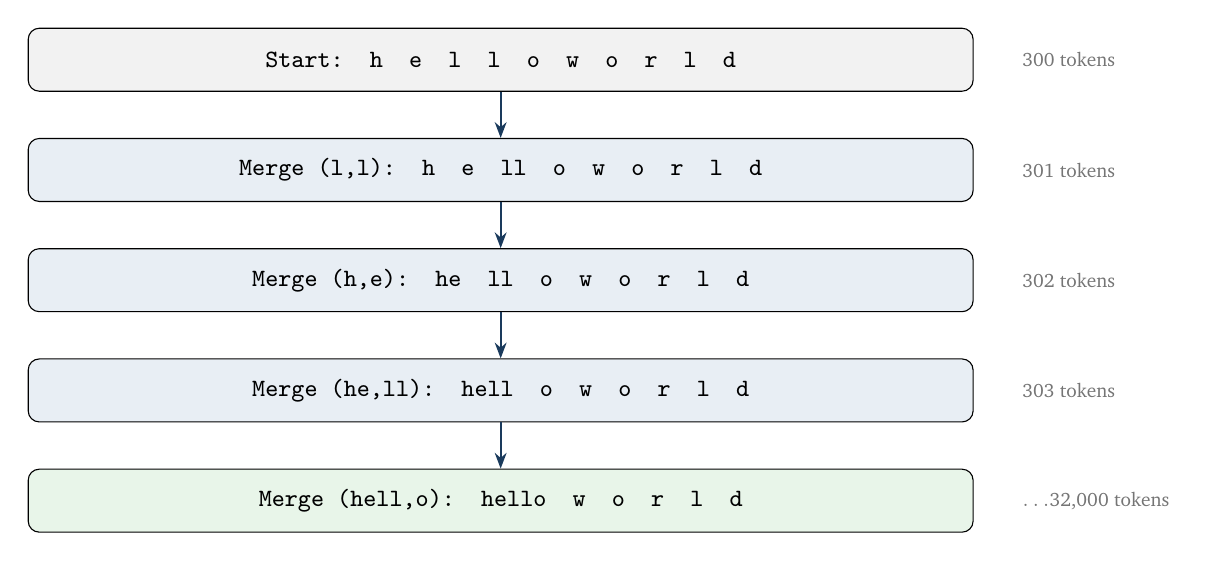
\begin{tikzpicture}[
    step/.style={draw, rounded corners, fill=#1, minimum width=12cm, minimum height=0.8cm, align=left, font=\small\ttfamily},
    arrow/.style={-{Stealth[length=2mm]}, thick, color=accent}
]
\node[step=gray!10] (s0) at (0, 0) {Start:\quad h~~e~~l~~l~~o~~w~~o~~r~~l~~d};
\node[step=lightaccent] (s1) at (0, -1.4) {Merge (l,l):\quad h~~e~~\textbf{ll}~~o~~w~~o~~r~~\textbf{l}~~d};
\node[step=lightaccent] (s2) at (0, -2.8) {Merge (h,e):\quad \textbf{he}~~ll~~o~~w~~o~~r~~l~~d};
\node[step=lightaccent] (s3) at (0, -4.2) {Merge (he,ll):\quad \textbf{hell}~~o~~w~~o~~r~~l~~d};
\node[step=tipbg] (s4) at (0, -5.6) {Merge (hell,o):\quad \textbf{hello}~~w~~o~~r~~l~~d};

\draw[arrow] (s0.south) -- (s1.north);
\draw[arrow] (s1.south) -- (s2.north);
\draw[arrow] (s2.south) -- (s3.north);
\draw[arrow] (s3.south) -- (s4.north);

\node[font=\scriptsize\color{codegray}, right] at (6.5, 0) {300 tokens};
\node[font=\scriptsize\color{codegray}, right] at (6.5, -1.4) {301 tokens};
\node[font=\scriptsize\color{codegray}, right] at (6.5, -2.8) {302 tokens};
\node[font=\scriptsize\color{codegray}, right] at (6.5, -4.2) {303 tokens};
\node[font=\scriptsize\color{codegray}, right] at (6.5, -5.6) {$\ldots$32,000 tokens};
\end{tikzpicture}
\caption{BPE builds tokens bottom-up by repeatedly merging the most frequent pair. Common words like ``hello'' eventually become single tokens, while rare words remain split into subwords.}
\label{fig:bpe}
\end{figure}

The beauty of BPE is that it is \textbf{data-driven}: it automatically discovers the most useful subwords for whatever languages are in the training data. Common words become single tokens, common prefixes and suffixes become tokens, and truly rare strings are broken into small pieces.

\subsection{The Critical Design Choice: Training Data Balance}

Here is where multilingual tokenization gets interesting. BPE learns its vocabulary from the training data you give it. If you feed it 90\% English and 10\% Hebrew, it will create a vocabulary that is excellent for English but fragments Hebrew badly---because English pairs will always be more common and get merged first.

\textbf{Our approach:} We train the tokenizer on an \textbf{equally balanced} sample---25\% from each language. This ensures that Hebrew character pairs get merged just as aggressively as English pairs, producing a vocabulary that works well for all four languages.

\begin{table}[H]
\centering
\begin{tabular}{lccc}
\toprule
\textbf{Script} & \textbf{Ours} & \textbf{Llama-2} & \textbf{HebrewGPT} \\
\midrule
Arabic script & 46.7\% & 0.2\% & 0.4\% \\
Hebrew script & 27.8\% & 0.1\% & 72.2\% \\
Latin script & 24.3\% & 80.9\% & 7.0\% \\
Other & 1.2\% & 18.8\% & 20.4\% \\
\bottomrule
\end{tabular}
\caption{Vocabulary composition by script. Llama-2 is 81\% Latin---almost useless for our target languages. HebrewGPT is 72\% Hebrew---great for Hebrew, terrible for Arabic and Persian. Ours balances all three scripts.}
\label{tab:vocab_composition}
\end{table}

Notice that Arabic script tokens (46.7\%) outnumber Hebrew tokens (27.8\%) in our vocabulary, even though each language gets 25\% of the training data. This is because Persian \emph{also} uses Arabic script (with minor additions), so both Arabic and Persian contribute to Arabic-script tokens.

\begin{warning}
You might worry that balancing the tokenizer hurts English performance---after all, English gets only 25\% of the tokenizer training data instead of nearly 100\% in Llama-2. In practice, the penalty is tiny: our tokenizer uses 1.54 tokens per English word versus Llama-2's 1.51. A 2\% overhead on English in exchange for 49--69\% improvement on three other languages is an excellent trade.
\end{warning}

\subsection{SentencePiece: The Implementation}

We use Google's \textbf{SentencePiece} library \citep{kudo2018sentencepiece} rather than implementing BPE from scratch. SentencePiece adds several practical features:

\begin{itemize}
    \item \textbf{Language-agnostic:} It operates on raw Unicode text, not pre-tokenized words. This is critical for languages like Chinese, Japanese, or Arabic where word boundaries are ambiguous.
    
    \item \textbf{Byte fallback:} If the tokenizer encounters a character it has never seen, it can fall back to encoding individual bytes. This means the tokenizer can handle \emph{any} text, even in languages not in the training data.
    
    \item \textbf{Normalization:} SentencePiece applies Unicode normalization (NFKC) to standardize different encodings of the same character. Arabic, for example, has multiple Unicode representations for some letters.
    
    \item \textbf{Special tokens:} We define special tokens for model control:\\[4pt]
    \begin{tabular}{ll}
    \texttt{<s>} & Beginning of sequence \\
    \texttt{</s>} & End of sequence \\
    \texttt{<pad>} & Padding (for batching sequences of different lengths) \\
    \texttt{<|user|>} & Start of user message (for instruction following) \\
    \texttt{<|assistant|>} & Start of model response \\
    \end{tabular}
\end{itemize}

\begin{reporef}
\textbf{Tokenizer training script:}\hfill\texttt{tokenizer/scripts/train\_tokenizer.py}\\
\textbf{Tokenizer configuration:}\hfill\texttt{tokenizer/config/tokenizer\_config.json}\\
\textbf{Fertility analysis results:}\hfill\texttt{tokenizer/artifacts/fertility\_report.json}\\
\textbf{Vocabulary statistics:}\hfill\texttt{tokenizer/artifacts/vocabulary\_stats.json}\\

The training script collects balanced samples from each language, trains SentencePiece, and produces the \texttt{.model} and \texttt{.vocab} files used during pretraining.
\end{reporef}

\subsection{Evaluating Your Tokenizer}

Once you have a tokenizer, how do you know it is good? We use two metrics:

\subsubsection{Fertility (Tokens per Word)}

\textbf{Fertility} measures how many tokens the tokenizer needs per word on average. Lower is better.

\begin{itemize}
    \item \textbf{Fertility = 1.0}: Every word is a single token (ideal but impossible for large vocabularies).
    \item \textbf{Fertility = 1.5}: Most words are one token, some common words need two pieces.
    \item \textbf{Fertility = 4.0}: Most words are split into many pieces (very inefficient).
\end{itemize}

For a well-designed multilingual tokenizer, you want fertility below 2.0 for all target languages. Our tokenizer achieves this for English (1.54), Hebrew (1.34), and Persian (1.52). Arabic (2.22) is slightly higher due to the language's morphological complexity.

\subsubsection{Bytes per Token}

\textbf{Bytes per token} measures how much raw text each token represents. Higher is better.

This metric is useful because different scripts use different numbers of bytes per character. Hebrew characters are 2 bytes in UTF-8, while English characters are 1 byte. Bytes per token normalizes across scripts:

\begin{itemize}
    \item Our tokenizer: Hebrew = 5.12 bytes/token
    \item Llama-2: Hebrew = 1.76 bytes/token
\end{itemize}

Our tokenizer packs 2.9$\times$ more Hebrew text into each token.

\subsection{Practical Impact: A Concrete Example}

Consider two short sentences and how different tokenizers handle them:

\textbf{Hebrew:} ``habina hamela'khutit meshane et ha'olam'' (Artificial intelligence is changing the world):
\begin{itemize}
    \item \textbf{Ours}: 4 tokens (whole-word segmentation)
    \item \textbf{Llama-2}: 18 tokens (character-level fragmentation)
    \item \textbf{HebrewGPT}: 5 tokens (comparable---Hebrew-optimized)
\end{itemize}

\textbf{Arabic:} ``asimat faransa hia baris'' (The capital of France is Paris):
\begin{itemize}
    \item \textbf{Ours}: 5 tokens (whole-word segmentation)
    \item \textbf{Llama-2}: 22 tokens (character-level fragmentation)
    \item \textbf{HebrewGPT}: 19 tokens (character-level fragmentation)
\end{itemize}

The difference is dramatic: 4--5 tokens versus 18--22. This means our model processes 4$\times$ more text per forward pass, learns 4$\times$ faster per training step, and provides 4$\times$ more context at inference.

\subsection{The Specialization Trade-off}

You might ask: why not use HebrewGPT's tokenizer? It achieves 1.26 tokens per Hebrew word---slightly better than ours (1.34). The answer is that HebrewGPT's tokenizer is a \textbf{specialist}: 72\% of its vocabulary is Hebrew script. It handles Hebrew beautifully but fragments Arabic (4.15 tokens/word) and Persian (4.51 tokens/word) as badly as Llama-2.

We need a \textbf{generalist}: a tokenizer that performs well across all four languages, even if it is not the absolute best for any single one.

\begin{figure}[H]
\centering
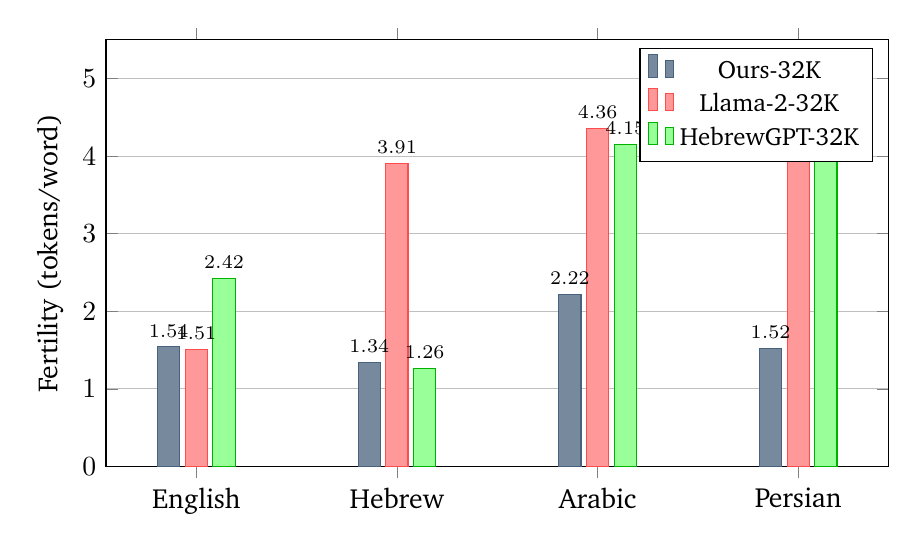
\begin{tikzpicture}
\begin{axis}[
    ybar,
    bar width=8pt,
    ylabel={Fertility (tokens/word)},
    symbolic x coords={English, Hebrew, Arabic, Persian},
    xtick=data,
    ymin=0, ymax=5.5,
    legend style={at={(0.98,0.98)}, anchor=north east, legend columns=1, font=\small},
    width=0.95\textwidth,
    height=7cm,
    ymajorgrids=true,
    enlarge x limits=0.15,
    nodes near coords,
    nodes near coords align={vertical},
    every node near coord/.append style={font=\scriptsize},
]
\addplot[fill=accent!60, draw=accent!80] coordinates {(English,1.54) (Hebrew,1.34) (Arabic,2.22) (Persian,1.52)};
\addplot[fill=red!40, draw=red!70] coordinates {(English,1.51) (Hebrew,3.91) (Arabic,4.36) (Persian,4.88)};
\addplot[fill=green!40, draw=green!70!black] coordinates {(English,2.42) (Hebrew,1.26) (Arabic,4.15) (Persian,4.51)};
\legend{Ours-32K, Llama-2-32K, HebrewGPT-32K}
\end{axis}
\end{tikzpicture}
\caption{Tokenizer fertility comparison (lower is better). Our tokenizer (blue) is the only one that performs well across \emph{all four} languages. Llama-2 (red) is good for English only. HebrewGPT (green) is good for Hebrew only.}
\label{fig:fertility_guide}
\end{figure}

\subsection{Summary: Building Your Own Tokenizer}

If you are building a multilingual model:

\begin{enumerate}
    \item \textbf{Do not reuse an English tokenizer.} The efficiency penalty on non-Latin scripts is severe (3--5$\times$).
    
    \item \textbf{Train on balanced data.} Equal language proportions during tokenizer training ensures fair vocabulary allocation.
    
    \item \textbf{Use SentencePiece BPE} with byte fallback and NFKC normalization.
    
    \item \textbf{Choose 32K--64K vocabulary} for 4--6 languages. Smaller vocabularies under-represent some languages; larger vocabularies waste embedding parameters.
    
    \item \textbf{Verify with fertility analysis.} Target $\leq$2.0 tokens per word for all languages. Check the English penalty---it should be minimal ($<$5\%).
    
    \item \textbf{Add special tokens} for your intended use case (instruction following, chat, etc.) \emph{before} training the tokenizer, so they get reserved IDs.
\end{enumerate}

\begin{tip}
Tokenizer training is fast (minutes, not hours) and does not require a GPU. You can iterate on the tokenizer many times, testing different vocabulary sizes and language balances, before committing to pretraining. This is one of the cheapest experiments you can run, so do not skimp on it.
\end{tip}

\begin{successcheck}
\begin{itemize}[nosep]
  \item Fertility $\leq$2.0 tokens per word for all target languages
  \item English penalty $<$5\% compared to an English-only tokenizer
  \item Vocabulary composition roughly reflects your language mix
  \item Encoding then decoding any test sentence produces the original text
  \item Special tokens (\texttt{<|user|>}, \texttt{<|assistant|>}) are in the vocabulary
\end{itemize}
\end{successcheck}

\begin{failuresign}
\begin{itemize}[nosep]
  \item Fertility $>$3.0 for any language --- vocabulary is too small or training data was unbalanced
  \item One language dominates $>$60\% of vocabulary --- retrain with equal-proportion data
  \item Characters from a target script are missing --- check your training data coverage
  \item Round-trip encoding/decoding loses characters --- byte fallback may be disabled
\end{itemize}
\end{failuresign}

% ============================================================
% CHAPTER 4: PLACEHOLDER
% ============================================================

\section{Collecting and Preparing Training Data}
\label{ch:data}

\begin{center}
\colorbox{lightaccent}{\textbf{Track: Concept + Build}}
\end{center}

A language model is only as good as the text it learns from. This chapter covers where to find multilingual training data, how to clean it, how to balance it across languages, and the practical decisions that shaped our 4.48-billion-token corpus.

\begin{warning}[title={Most Beginner Failures Start Here}]
Data problems are the \#1 cause of failed training runs. Inverted labels, sorted datasets, data leakage, and low-quality sources all produce models that \emph{appear} to work but give meaningless results. If you skip one chapter's verification steps, do not skip this one's.
\end{warning}

\begin{buildnow}
\textbf{Outcome:} A clean, tokenized, balanced corpus stored as binary files with manifests tracking every source.

\textbf{Decisions required:}
\begin{itemize}[nosep]
  \item Which data sources for each language
  \item Language balance proportions (e.g., 40/20/20/20)
  \item Quality filtering thresholds
\end{itemize}

\textbf{Safe defaults:} Wikipedia + OSCAR per language, anchor language at 40\%, others equal. MinHash dedup, language-ID filtering.

\textbf{Skip on first pass:} Perplexity-based filtering (\S4.4 quality section). Start with language-ID filtering only.
\end{buildnow}

The data pipeline has five numbered stages:
\begin{enumerate}[nosep]
  \item \textbf{Collect} --- download raw text from multiple sources per language.
  \item \textbf{Clean} --- deduplicate, run language ID, apply quality filters.
  \item \textbf{Tokenize} --- convert to token IDs using your custom tokenizer.
  \item \textbf{Mix} --- combine language files to target proportions.
  \item \textbf{Verify} --- spot-check decoded examples, confirm token counts and language balance.
\end{enumerate}

\subsection{How Much Data Do You Need?}

The relationship between model size and training data is governed by \textbf{scaling laws}---empirical findings about how much data a model of a given size needs to train optimally. The most cited rule of thumb comes from the Chinchilla paper (Hoffmann et al., 2022): a model should be trained on roughly 20$\times$ its parameter count in tokens.

For our 3.14B parameter model, that suggests:
$$3.14\text{B} \times 20 = 62.8\text{B tokens (optimal)}$$

We trained on 4.48B tokens---about 14$\times$ less than the Chinchilla-optimal amount. Why?

\begin{enumerate}
    \item \textbf{Data availability.} For Hebrew, high-quality text simply does not exist at the 60B-token scale. You cannot train on data you do not have.
    \item \textbf{Budget constraints.} Training on 62B tokens would take roughly 14$\times$ longer (and cost 14$\times$ more). Our goal was a research model, not a production one.
    \item \textbf{Diminishing returns at small scale.} Scaling laws assume you are pushing frontier performance. For our research questions about cross-lingual transfer, 4.48B tokens proved sufficient to demonstrate the phenomena.
\end{enumerate}

\begin{keyidea}
For low-resource languages, you are almost always \textbf{data-limited, not compute-limited}. The bottleneck is finding enough clean text in your target languages, not buying enough GPUs. This makes data collection and quality the most important phase of the project.
\end{keyidea}

\subsection{Where to Find Multilingual Text}

Our corpus draws from several public sources. Here is what is available and what we used:

\subsubsection{Wikipedia}

\textbf{What it is:} Free encyclopedia articles in 300+ languages.\\
\textbf{Quality:} High---edited, factual, formal register.\\
\textbf{Size:} Small for most languages. Hebrew Wikipedia is about 1.2 GB of raw text; Arabic is about 2.1 GB.\\
\textbf{License:} CC-BY-SA (free to use with attribution).\\
\textbf{Where to get it:} \url{https://dumps.wikimedia.org/}

Wikipedia is a good foundation but nowhere near sufficient on its own. It represents only one style (encyclopedic) and is relatively small.

\subsubsection{OSCAR}

\textbf{What it is:} A massive multilingual web crawl, filtered by language. Part of the Common Crawl ecosystem.\\
\textbf{Quality:} Variable---ranges from clean news articles to near-gibberish. Requires filtering.\\
\textbf{Size:} Large. Hebrew OSCAR is about 8 GB; Arabic is about 12 GB.\\
\textbf{License:} CC-BY-4.0.\\
\textbf{Where to get it:} \url{https://oscar-project.org/}

OSCAR provides the bulk of our training data. The trade-off is volume versus quality: you get a lot of text, but you must invest in cleaning it.

\subsubsection{News Corpora}

\textbf{What it is:} Collections of news articles from various publications.\\
\textbf{Quality:} High---professionally written, diverse topics.\\
\textbf{Size:} Medium. Typically 1--5 GB per language.\\
\textbf{License:} Varies; often ``research only.''

News text provides valuable formal-register content and topical diversity.

\subsubsection{Government Documents}

For Hebrew specifically, Israeli government publications, Knesset proceedings, and legal texts provide high-quality formal Hebrew. These are often overlooked but are usually publicly available.

\subsubsection{Parallel Corpora (for Translation)}

For our supervised fine-tuning phase (Chapter~\ref{ch:sft}), we also need \textbf{parallel text}---the same content in two languages, sentence-aligned. Our primary source is \textbf{OPUS-100} \citep{zhang2020improving}, which provides millions of sentence pairs for many language combinations.

\begin{warning}
Not all language pairs are available in parallel corpora. OPUS-100 has English$\leftrightarrow$Hebrew, English$\leftrightarrow$Arabic, and English$\leftrightarrow$Persian, but \emph{not} Hebrew$\leftrightarrow$Arabic or Hebrew$\leftrightarrow$Persian directly. This is a common limitation for low-resource language pairs.
\end{warning}

\subsection{Our Data Distribution: The Anchor Language Strategy}

We do not split data equally across languages. Instead, we use an \textbf{anchor language} strategy, overrepresenting Hebrew:

\begin{table}[H]
\centering
\begin{tabular}{lrrl}
\toprule
\textbf{Language} & \textbf{Share} & \textbf{$\sim$Tokens} & \textbf{Rationale} \\
\midrule
Hebrew & 40\% & 1.79B & Anchor language---strongest representations \\
Arabic & 20\% & 0.90B & Semitic sibling to Hebrew \\
English & 20\% & 0.90B & High-resource bridge language \\
Persian & 20\% & 0.90B & Typological control (Indo-European) \\
\midrule
\textbf{Total} & 100\% & \textbf{4.48B} & \\
\bottomrule
\end{tabular}
\caption{Pretraining data distribution. Hebrew receives 2$\times$ the share of other languages to establish strong anchor representations.}
\label{tab:data_dist}
\end{table}

Why overrepresent Hebrew? The idea is that by giving one language extra data, the model builds especially strong internal representations for it. If cross-lingual transfer works, those strong Hebrew representations might ``pull up'' related languages (especially Arabic, which shares Semitic roots) during training. Whether this actually works better than equal distribution is an open question---we did not ablate it---but the strategy is common in multilingual modeling.

\begin{tip}
Note that the tokenizer is trained on equal 25\% shares, but the \emph{pretraining data} uses 40/20/20/20. These are independent decisions. The tokenizer balance ensures fair vocabulary; the data balance determines how much each language is learned during pretraining.
\end{tip}

\subsection{Data Cleaning: Turning Raw Text into Training Data}

Raw web text is messy. Here are the cleaning steps we apply, and why each matters:

\subsubsection{Deduplication (MinHash)}

\textbf{Problem:} Web crawls contain enormous amounts of duplicate content---the same article republished on dozens of sites, boilerplate headers/footers, cookie notices repeated on every page.

\textbf{Solution:} \textbf{MinHash deduplication} creates a compact ``fingerprint'' of each document and efficiently finds near-duplicates. Documents that are more than $\sim$80\% similar to an existing document are removed.

\textbf{Why it matters:} Duplicate data causes the model to memorize specific texts rather than learning general patterns. It also wastes training compute on content the model has already seen.

\subsubsection{Language Identification}

\textbf{Problem:} OSCAR and other web corpora are filtered by language, but the filtering is imperfect. A ``Hebrew'' document might actually be in Russian, or might be mostly English with a few Hebrew words.

\textbf{Solution:} Run a language identification model (such as FastText's \texttt{lid.176.bin}) on each document and discard documents where the detected language does not match the expected language.

\textbf{Why it matters:} Training on mislabeled data confuses the model about what each language looks like.

\subsubsection{Perplexity-Based Quality Filtering}

\textbf{Problem:} Some documents are technically in the right language but are very low quality---machine-generated text, SEO spam, random word salad, or text extraction artifacts.

\textbf{Solution:} Train a small language model on known-good text (e.g., Wikipedia) and use it to score each document's \textbf{perplexity}---how ``surprised'' the model is by the text. Discard documents with very high perplexity (the model finds them incomprehensible) or very low perplexity (likely repetitive boilerplate).

\textbf{Why it matters:} Quality filtering has a larger impact on downstream performance than simply adding more data. A smaller clean dataset often beats a larger noisy one.

\subsubsection{Additional Cleaning}

\begin{itemize}
    \item \textbf{HTML/boilerplate removal:} Strip remaining HTML tags, navigation menus, and page templates.
    \item \textbf{Length filtering:} Remove documents shorter than 50 characters (likely fragments) or extremely long single-paragraph documents (likely extraction errors).
    \item \textbf{Personal information:} Remove email addresses, phone numbers, and other PII where detected.
    \item \textbf{Unicode normalization:} Standardize different Unicode representations of the same character (important for Arabic script, which has multiple forms).
\end{itemize}

\subsection{Tokenization: From Clean Text to Training Files}

Once the text is clean, we run it through our tokenizer (Chapter~\ref{ch:tokenizer}) to convert it from human-readable text into sequences of token IDs---integers between 0 and 31,999.

The tokenized data is stored as \textbf{binary files} of unsigned 16-bit integers (\texttt{uint16}), one per token. This is compact (2 bytes per token) and fast to read during training. A 4.48B-token dataset takes about 8.96 GB on disk in this format.

During training, the data loader reads these binary files and constructs training examples by slicing them into fixed-length sequences of 2,048 tokens. No padding is needed because the binary format is contiguous---the end of one document flows into the beginning of the next, separated by end-of-sequence tokens.

\subsection{Data Manifests: Tracking What You Have}

With data coming from multiple sources in multiple languages, organization is critical. We maintain \textbf{manifests}---JSON files that record exactly what is in the dataset:

\begin{itemize}
    \item \textbf{Source manifest:} For each language, lists every data source with its URL, estimated size, type (encyclopedia, web crawl, news), and license.
    \item \textbf{Mixture specification:} Records the target proportions for each language and the mixing strategy.
    \item \textbf{Training data metadata:} Records the actual token counts after processing, checksums, and creation dates.
\end{itemize}

This may seem like bureaucratic overhead, but it is essential for reproducibility and debugging. When your model behaves unexpectedly on Arabic (as ours did---see Chapter~\ref{ch:lessons}), you need to be able to trace exactly what Arabic data it trained on.

\begin{reporef}
\textbf{Data collection scripts:}\hfill\texttt{data/scripts/}\\
\quad\texttt{collect\_native\_data\_v2.py}\hfill Main collection pipeline\\
\quad\texttt{arabic\_collect.py}\hfill Arabic-specific collection\\
\quad\texttt{farsi\_collect.py}\hfill Persian-specific collection\\
\quad\texttt{collect\_translation\_data\_v2.py}\hfill Parallel corpus collection\\
\quad\texttt{retokenize\_arabic.py}\hfill Arabic retokenization after rebalancing\\
[6pt]
\textbf{Data manifests:}\hfill\texttt{data/manifests/}\\
\quad\texttt{source\_manifest.json}\hfill All data sources with URLs and licenses\\
\quad\texttt{mixture\_spec.json}\hfill Language proportions\\
\quad\texttt{training\_data\_metadata.json}\hfill Final token counts and checksums\\
\end{reporef}

\subsection{Summary: The Data Pipeline}

Here is the complete pipeline from raw sources to training-ready data:

\begin{figure}[H]
\centering
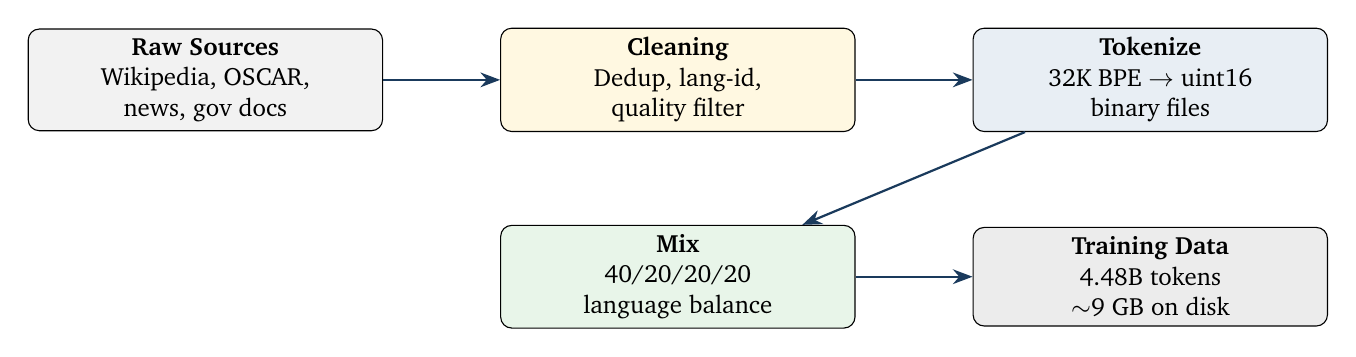
\begin{tikzpicture}[
    box/.style={draw, rounded corners, fill=#1, minimum width=4.5cm, minimum height=1cm, align=center, font=\small},
    arrow/.style={-{Stealth[length=2.5mm]}, thick, color=accent}
]
\node[box=gray!10] (raw) at (0, 0) {\textbf{Raw Sources}\\Wikipedia, OSCAR,\\news, gov docs};
\node[box=warnbg] (clean) at (6, 0) {\textbf{Cleaning}\\Dedup, lang-id,\\quality filter};
\node[box=lightaccent] (tok) at (12, 0) {\textbf{Tokenize}\\32K BPE $\rightarrow$ uint16\\binary files};
\node[box=tipbg] (mix) at (6, -2.5) {\textbf{Mix}\\40/20/20/20\\language balance};
\node[box=gray!15] (train) at (12, -2.5) {\textbf{Training Data}\\4.48B tokens\\$\sim$9 GB on disk};

\draw[arrow] (raw) -- (clean);
\draw[arrow] (clean) -- (tok);
\draw[arrow] (tok) -- (mix);
\draw[arrow] (mix) -- (train);
\end{tikzpicture}
\caption{The data pipeline. Each step reduces volume but increases quality. The final output is a compact binary file ready for the training loop.}
\label{fig:data_pipeline}
\end{figure}

\begin{enumerate}
    \item \textbf{Collect} raw text from multiple sources per language.
    \item \textbf{Clean} with deduplication, language ID, and quality filtering.
    \item \textbf{Tokenize} with your custom multilingual tokenizer.
    \item \textbf{Mix} according to your target language proportions.
    \item \textbf{Store} as compact binary files with manifests for tracking.
    \item \textbf{Verify} token counts, language proportions, and data integrity before training.
\end{enumerate}

\begin{tip}
Invest in data quality \emph{before} you start training. Once pretraining begins, it is extremely expensive to restart because you discovered a data problem. We spent roughly one week on data collection and cleaning versus one day on actual pretraining. That ratio is typical and appropriate.
\end{tip}

\begin{successcheck}
\begin{itemize}[nosep]
  \item Token counts per language match your target proportions ($\pm$2\%)
  \item Decoded spot-checks (100+ per language) show clean, natural text in the correct language
  \item Manifest files record every source, its license, and processing steps
  \item No duplicate documents remain after dedup
  \item Binary files load correctly and produce valid token IDs
\end{itemize}
\end{successcheck}

\begin{failuresign}
\begin{itemize}[nosep]
  \item One language has $<$10\% of expected tokens --- download or filtering failed silently
  \item Decoded text contains HTML tags, URLs, or boilerplate --- cleaning filters are too permissive
  \item Language-ID check shows $>$5\% mislabeled documents --- source quality is poor
  \item File sizes are unexpectedly small (e.g., 4 KB instead of 400 MB) --- download or conversion failed
\end{itemize}
\end{failuresign}

% ============================================================
% CHAPTER 5: PLACEHOLDER
% ============================================================

\section{Proxy Experiments: Testing Before Committing}
\label{ch:proxy}

\begin{center}
\colorbox{lightaccent}{\textbf{Track: Concept + Build}}
\end{center}

Pretraining a 3B model costs real money and takes real time. If your training recipe is wrong---bad learning rate, wrong optimizer, broken schedule---you will not discover this until hours or days into the run, by which point you have wasted the entire investment. \textbf{Proxy experiments} solve this by testing your recipe at small scale first.

\begin{buildnow}
\textbf{Outcome:} A validated training recipe (optimizer, LR, schedule, weight decay) tested at 110M scale.

\textbf{Decisions required:}
\begin{itemize}[nosep]
  \item Proxy model size (typically 25--30$\times$ smaller than full)
  \item Which hyperparameters to sweep
  \item How many experiments to run (20--40 minimum)
\end{itemize}

\textbf{Safe defaults:} 110M proxy for a 3B target. AdamW optimizer, cosine LR schedule, peak LR 3e-4, weight decay 0.1.

\textbf{Skip on first pass:} Exotic optimizers (Muon, etc.). Start with AdamW---it never diverges.
\end{buildnow}

\subsection{The Idea}

A proxy experiment is a miniature version of your full training run. Instead of training a 3B model on 4.48B tokens (22 hours on 8 GPUs), you train a 110M model on a few hundred million tokens (2--5 minutes on 1 GPU). The hypothesis is that a recipe that works well at small scale will also work well at large scale. This is not always true, but it is true often enough to be extremely useful.

\begin{keyidea}
Proxy experiments let you explore 30+ recipe variations in the time it takes to run one full training job. We ran \textbf{32 proxy experiments} to select our final training recipe before committing to the 3B pretraining run. Total cost: roughly 16 GPU-hours on a single L40S. The full run cost 180 GPU-hours on 8$\times$H100. The proxy experiments were less than 1\% of the cost but eliminated the most dangerous recipe risks.
\end{keyidea}

\subsection{What We Tested}

Our proxy experiments explored six dimensions of the training recipe:

\begin{table}[H]
\centering
\begin{tabular}{clp{6cm}}
\toprule
\textbf{Priority} & \textbf{Sweep Variable} & \textbf{Why This Order} \\
\midrule
1 & LR schedule shape & Determines the overall training trajectory \\
2 & Optimizer (AdamW vs.\ exotic) & Must be stable before tuning other knobs \\
3 & Peak learning rate & Largest effect on convergence speed \\
4 & Weight decay & Regularization; moderate effect \\
5 & Warmup duration & Minor effect if LR schedule is correct \\
6 & Batch size & Usually hardware-constrained; tune last \\
\bottomrule
\end{tabular}
\caption{Recommended sweep order. Test variables in this order; each row assumes prior rows are fixed.}
\end{table}

\begin{tip}[title={Your First 10 Proxy Experiments}]
If you have time for only 10 experiments, run these:
\begin{enumerate}[nosep]
  \item Cosine schedule + AdamW + LR 1e-3 (baseline)
  \item Cosine schedule + AdamW + LR 3e-4
  \item Cosine schedule + AdamW + LR 5e-4
  \item Cosine schedule + AdamW + LR 1e-4
  \item Linear schedule + AdamW + LR 3e-4
  \item Cosine + AdamW + LR 3e-4 + weight decay 0.05
  \item Cosine + AdamW + LR 3e-4 + weight decay 0.2
  \item Cosine + AdamW + LR 3e-4 + 500-step warmup
  \item Cosine + AdamW + LR 3e-4 + 2000-step warmup
  \item Best config from above, run 2$\times$ longer to check stability
\end{enumerate}
This covers the highest-impact variables. Expand from here if time allows.
\end{tip}

\subsubsection{1. Learning Rate Schedule}

The \textbf{learning rate} controls how much the model updates its parameters at each training step. Too high and training becomes unstable (loss explodes). Too low and training is too slow (loss barely decreases). The \textbf{schedule} controls how the learning rate changes over the course of training.

We tested four schedule types:

\begin{itemize}
    \item \textbf{Cosine decay}: Starts at peak LR, smoothly decreases following a cosine curve to near zero. This is the most common choice.
    \item \textbf{Warmup-Stable-Decay (WSD)}: Ramps up, holds constant for most of training, then linearly decays in the final 20\%. Often more robust than cosine.
    \item \textbf{Linear decay}: Simple ramp down from peak to zero.
    \item \textbf{Cosine with warm restarts}: Multiple cosine cycles, periodically resetting the learning rate. This is what our initial (failed) 1B run used.
\end{itemize}

\begin{figure}[H]
\centering
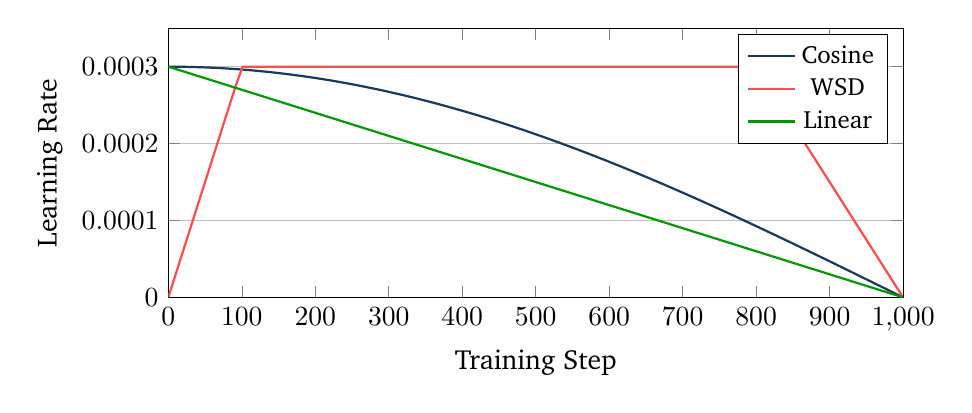
\begin{tikzpicture}
\begin{axis}[
    width=0.9\textwidth,
    height=5cm,
    xlabel={Training Step},
    ylabel={Learning Rate},
    xmin=0, xmax=1000,
    ymin=0, ymax=3.5e-4,
    legend style={at={(0.98,0.98)}, anchor=north east, font=\small},
    ymajorgrids=true,
    scaled y ticks=false,
    yticklabel style={/pgf/number format/fixed, /pgf/number format/precision=4},
]
\addplot[accent, thick, domain=0:1000, samples=100] {3e-4 * cos(deg(x/1000*pi/2))};
\addplot[red!70, thick, domain=0:1000, samples=100] {
    (x < 100) * (3e-4 * x / 100) +
    (x >= 100) * (x < 800) * 3e-4 +
    (x >= 800) * (3e-4 * (1 - (x-800)/200))
};
\addplot[green!60!black, thick, domain=0:1000, samples=100] {3e-4 * (1 - x/1000)};
\legend{Cosine, WSD, Linear}
\end{axis}
\end{tikzpicture}
\caption{Three learning rate schedules. Cosine (blue) decays smoothly throughout. WSD (red) holds the learning rate steady for most of training, then decays sharply at the end. Linear (green) decays at a constant rate. Our final recipe uses cosine decay.}
\label{fig:lr_schedules}
\end{figure}

\subsubsection{2. Optimizer Choice}

The \textbf{optimizer} is the algorithm that uses gradients (how wrong the model was) to update parameters (making the model less wrong). The two main contenders:

\begin{itemize}
    \item \textbf{AdamW} \citep{loshchilov2019adamw}: The standard optimizer for training transformers. Maintains running averages of gradients and their squares to adapt the learning rate per-parameter. The ``W'' means it applies weight decay correctly (a regularization technique that prevents parameters from growing too large).
    \item \textbf{Muon}: A newer optimizer that operates differently on different parameter shapes. Potentially faster convergence, but less tested and harder to tune.
\end{itemize}

Our proxy experiments started with Muon (which had been used in our earlier 1B attempt) but found it unstable at the learning rates we needed. We switched to AdamW for reliability.

\subsubsection{3. Peak Learning Rate}

We tested peak learning rates from 1e-4 to 8e-4. Our final choice: \textbf{3e-4}, which is a common default for AdamW with transformer models. Higher rates trained faster initially but sometimes caused instability; lower rates were more stable but slower.

\subsubsection{4. Training Duration (Steps)}

How long should you train? We tested runs from 200 to 2000 proxy steps (equivalent to different amounts of data). The key finding: validation loss kept improving through our entire proxy range, with no sign of overfitting. This gave us confidence that the full 20,000-step run would not overtrain.

\subsubsection{5. Weight Decay}

\textbf{Weight decay} is a regularization technique that gently pushes all parameters toward zero, preventing any single parameter from becoming too large. We tested values from 0.01 to 0.1. Our final choice: \textbf{0.1}, which is aggressive but standard for large language models.

\subsubsection{6. Stochastic Weight Averaging (SWA)}

\textbf{SWA} maintains a running average of the model's parameters over the last portion of training. The averaged model is often slightly better than any single checkpoint because it smooths out the noise of individual training steps. We tested starting SWA at the last 10\%, 20\%, and 30\% of training.

\subsection{The Proxy Architecture}

Our proxy model is a scaled-down version of the full architecture:

\begin{table}[H]
\centering
\begin{tabular}{lcc}
\toprule
\textbf{Parameter} & \textbf{Proxy (110M)} & \textbf{Full (3.14B)} \\
\midrule
Hidden dimension & 768 & 3,072 \\
Layers & 12 & 26 \\
Attention heads & 12 & 24 \\
Training steps & 200--2,000 & 20,000 \\
Time per run & 2--5 minutes & 22.4 hours \\
GPU & 1$\times$ L40S & 8$\times$ H100 \\
\bottomrule
\end{tabular}
\caption{Proxy vs.\ full model. The proxy is $\sim$28$\times$ smaller and trains $\sim$250$\times$ faster, enabling rapid iteration.}
\label{tab:proxy_vs_full}
\end{table}

The proxy uses the same tokenizer, same data, same optimizer, and same code---just smaller dimensions. This maximizes the chance that findings transfer to the full scale.

\subsection{What We Found}

Across 32 experiments, here are the key findings:

\begin{enumerate}
    \item \textbf{AdamW beats Muon for reliability.} Muon showed promising early convergence but was sensitive to learning rate and caused training explosions in 3 of 8 runs. AdamW never diverged.
    \item \textbf{Cosine schedule slightly outperformed WSD.} Both worked well, but cosine was more consistent across different learning rates.
    \item \textbf{Peak LR of 3e-4 was optimal.} 5e-4 was faster but occasionally unstable. 1e-4 was too slow.
    \item \textbf{SWA helped modestly.} Starting at the last 20\% of training gave small but consistent improvements.
    \item \textbf{Label smoothing and gradient scaling were unnecessary.} Both added complexity without improving results on bf16 hardware.
\end{enumerate}

\begin{reporef}
\textbf{Proxy experiment framework:}\hfill\texttt{proxy/}\\
\quad\texttt{train.py}\hfill Proxy training script\\
\quad\texttt{run\_agent.py}\hfill Autonomous experiment runner\\
\quad\texttt{setup\_and\_run.sh}\hfill Environment setup\\
\quad\texttt{program.md}\hfill Experiment program (what to test and why)\\
[4pt]
\textbf{Experiment configs:}\hfill\texttt{proxy/configs/}\\
\quad\texttt{exp\_000\_train.py} through \texttt{exp\_032\_train.py}\hfill All 32 configurations\\
[4pt]
\textbf{Results:}\hfill\texttt{proxy/results/}\\
\quad\texttt{results.tsv}\hfill All results in tabular format\\
\quad\texttt{muon\_arch\_results.log}\hfill Muon vs.\ AdamW comparison\\
\quad\texttt{tokenizer\_training\_results.json}\hfill Tokenizer variant results\\
[4pt]
\textbf{Recipe rationale:}\hfill\texttt{proxy/rationale/recipe\_selection.md}
\end{reporef}

\subsection{Lessons for Your Own Proxy Experiments}

\begin{enumerate}
    \item \textbf{Keep the proxy as similar to the full run as possible.} Same code, same data, same tokenizer. Only change the model size and training duration.
    \item \textbf{Use a consistent evaluation metric.} We used validation BPB (bits per byte) measured on a held-out set. Compare all experiments on the same metric.
    \item \textbf{Test one variable at a time when possible.} If you change both the optimizer and the learning rate, you will not know which caused the improvement.
    \item \textbf{Run failing experiments too.} Some of our most useful findings came from understanding \emph{why} an experiment failed (e.g., Muon divergence at high LR).
    \item \textbf{Budget 10--20 proxy runs minimum.} Fewer than that and you are guessing. More than 50 and you are probably over-optimizing for the proxy scale.
\end{enumerate}

\begin{tip}
Proxy experiments are also excellent for testing data pipeline changes. If you suspect your Arabic data has quality issues, run a proxy with and without Arabic and compare. This takes 5 minutes instead of discovering the problem 15 hours into a full run.
\end{tip}

\begin{successcheck}
\begin{itemize}[nosep]
  \item Your best configuration shows monotonically decreasing validation BPB
  \item At least 20 experiments completed without divergence
  \item A clear winner emerges (not a tie between very different configs)
  \item All results are documented with configs and rationale
  \item The winning recipe uses a ``boring'' optimizer (AdamW) that never diverged
\end{itemize}
\end{successcheck}

\begin{failuresign}
\begin{itemize}[nosep]
  \item Multiple experiments diverge (loss explodes) --- learning rate is too high or optimizer is unstable
  \item Validation BPB plateaus early --- learning rate may be too low or schedule decays too fast
  \item Results vary wildly between runs with same config --- training is not deterministic; check random seeds
  \item You ran $<$10 experiments --- you are guessing, not validating
\end{itemize}
\end{failuresign}


% ============================================================
% CHAPTER 6: PRETRAINING
% ============================================================

\section{Pretraining: Teaching the Model to Read}
\label{ch:pretraining}

\begin{center}
\colorbox{tipbg}{\textbf{Track: Build}}
\end{center}

Pretraining is where the model learns language. You feed it billions of tokens of raw text, and through the simple task of predicting the next token, it learns grammar, vocabulary, facts, and---crucially for our purposes---cross-lingual structure. This is the most expensive phase of the project and the one where mistakes are most costly.

\begin{buildnow}
\textbf{Outcome:} A pretrained model checkpoint with monotonically decreasing validation loss.

\textbf{Decisions required:}
\begin{itemize}[nosep]
  \item GPU instance type and count
  \item FSDP sharding strategy and mixed-precision settings
  \item Checkpoint frequency and storage location
\end{itemize}

\textbf{Safe defaults:} Use exactly the recipe validated by proxy experiments. FSDP with bf16 compute / fp32 reduce. Checkpoints every 250 steps to S3.

\textbf{Skip on first pass:} Advanced monitoring dashboards. Watch loss, BPB, and TPS in the terminal.
\end{buildnow}

\subsection{What Happens During Pretraining}

At a high level, each training step works like this:

\begin{enumerate}
    \item \textbf{Load a batch.} Pull a batch of text sequences from the training data. Each sequence is 2,048 tokens long. With our batch size of 512K tokens, that is 250 sequences per step.
    \item \textbf{Forward pass.} Feed the batch through the model. For each position in each sequence, the model predicts what the next token should be.
    \item \textbf{Compute loss.} Compare the model's predictions to the actual next tokens. The \textbf{cross-entropy loss} measures how wrong the model was---lower is better.
    \item \textbf{Backward pass.} Compute \textbf{gradients}: for each of the 3.14 billion parameters, calculate how much changing that parameter would reduce the loss. This is done automatically by PyTorch's autograd system.
    \item \textbf{Update parameters.} The optimizer (AdamW) uses the gradients to adjust each parameter slightly. The learning rate controls how large these adjustments are.
    \item \textbf{Repeat.} Go back to step 1. Our training runs for 20,000 steps.
\end{enumerate}

\begin{figure}[H]
\centering
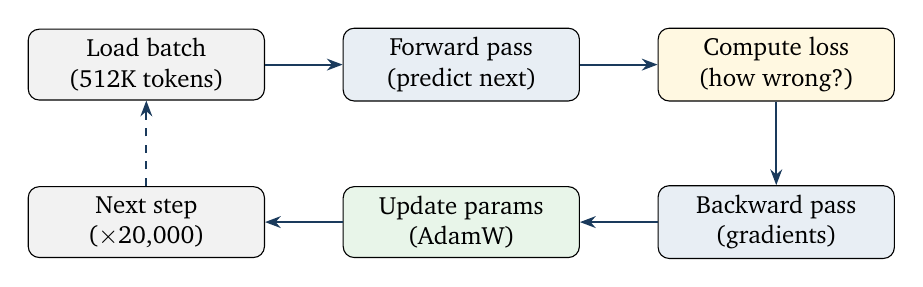
\begin{tikzpicture}[
    box/.style={draw, rounded corners, fill=#1, minimum width=3cm, minimum height=0.9cm, align=center, font=\small},
    arrow/.style={-{Stealth[length=2mm]}, thick, color=accent}
]
\node[box=gray!10] (load) at (0, 0) {Load batch\\(512K tokens)};
\node[box=lightaccent] (fwd) at (4, 0) {Forward pass\\(predict next)};
\node[box=warnbg] (loss) at (8, 0) {Compute loss\\(how wrong?)};
\node[box=lightaccent] (bwd) at (8, -2) {Backward pass\\(gradients)};
\node[box=tipbg] (update) at (4, -2) {Update params\\(AdamW)};
\node[box=gray!10] (next) at (0, -2) {Next step\\($\times$20,000)};

\draw[arrow] (load) -- (fwd);
\draw[arrow] (fwd) -- (loss);
\draw[arrow] (loss) -- (bwd);
\draw[arrow] (bwd) -- (update);
\draw[arrow] (update) -- (next);
\draw[arrow, dashed] (next) -- (load);
\end{tikzpicture}
\caption{The training loop. Each of 20,000 steps processes 512K tokens. Over the full run, the model sees 4.48B tokens.}
\label{fig:training_loop}
\end{figure}

\subsection{Distributed Training with FSDP}

Our model has 3.14 billion parameters. In bfloat16 precision, each parameter takes 2 bytes. So the model itself is $\sim$6.3 GB. But during training, we also need:

\begin{itemize}
    \item \textbf{Gradients:} One gradient per parameter ($\sim$6.3 GB)
    \item \textbf{Optimizer states:} AdamW stores two running averages per parameter ($\sim$12.6 GB in float32)
    \item \textbf{Activations:} Intermediate values saved for the backward pass ($\sim$10--20 GB depending on batch size)
\end{itemize}

Total memory: roughly 35--45 GB. A single H100 has 80 GB of memory, so technically it fits, but the batch size would be tiny. To train efficiently, we distribute across \textbf{8 GPUs} using a technique called \textbf{FSDP (Fully Sharded Data Parallelism)} \citep{zhao2023fsdp}.

\subsubsection{How FSDP Works}

Imagine you have 8 GPUs, each with 80 GB of memory. Without FSDP, each GPU holds a \emph{complete copy} of the model plus optimizer states, wasting 7/8 of the total memory on redundant copies.

FSDP \textbf{shards} (splits) the model across GPUs. Each GPU holds only 1/8 of the parameters, 1/8 of the gradients, and 1/8 of the optimizer states. When a layer needs the full parameters for computation, FSDP temporarily gathers them from all GPUs, computes, and then discards the non-local copies.

\begin{table}[H]
\centering
\begin{tabular}{lcc}
\toprule
\textbf{Component} & \textbf{Without FSDP} & \textbf{With FSDP} \\
 & (per GPU) & (per GPU) \\
\midrule
Model parameters & 6.3 GB & 0.8 GB \\
Gradients & 6.3 GB & 0.8 GB \\
Optimizer states & 12.6 GB & 1.6 GB \\
Activations & $\sim$15 GB & $\sim$15 GB \\
\midrule
\textbf{Total} & $\sim$40 GB & $\sim$18 GB \\
\bottomrule
\end{tabular}
\caption{Memory usage per GPU with and without FSDP (8 GPUs). FSDP reduces per-GPU memory by more than half, allowing larger batch sizes or larger models.}
\label{tab:fsdp_memory}
\end{table}

The trade-off is \textbf{communication}: FSDP must send parameter shards between GPUs before and after each layer's computation. On modern hardware with fast interconnects (like the NVLink in our p5en node), this overhead is small---typically 5--15\% of total training time.

\subsubsection{Mixed Precision: bfloat16}

Training in full 32-bit floating point (float32) would double all the memory numbers above. Instead, we use \textbf{bfloat16} (brain floating-point 16), a format that uses half the memory while maintaining the same dynamic range as float32.

The key properties of bfloat16:
\begin{itemize}
    \item \textbf{16 bits} instead of 32 $\rightarrow$ half the memory, roughly 2$\times$ faster computation.
    \item \textbf{Same exponent range as float32} $\rightarrow$ can represent very large and very small numbers.
    \item \textbf{Less precision in the mantissa} $\rightarrow$ slightly noisier computations, but this rarely matters in practice.
\end{itemize}

We use bfloat16 for the forward and backward passes (where speed matters most) and float32 for the optimizer state updates (where numerical precision matters most). This is called \textbf{mixed precision} training.

\begin{tip}
bfloat16 is only available on relatively modern GPUs (NVIDIA A100, H100, L40S, and newer). Older GPUs (V100, T4) support float16 instead, which has a narrower dynamic range and requires more careful loss scaling. If you are using older hardware, you will need a \texttt{GradScaler}---but on modern hardware, bfloat16 ``just works.''
\end{tip}

\subsection{Training Configuration}

Here is our complete training configuration, with explanations:

\begin{table}[H]
\centering
\begin{tabular}{llp{6.5cm}}
\toprule
\textbf{Parameter} & \textbf{Value} & \textbf{Why} \\
\midrule
Optimizer & AdamW & Reliable, well-understood. Validated in proxy experiments over Muon. \\
Peak learning rate & 3e-4 & Standard for this model size. Validated in proxy. \\
LR schedule & Cosine decay & Smooth decay, slight edge over WSD in proxy. \\
Warmup & 2,000 steps & Gradual ramp-up prevents early instability. 10\% of total steps. \\
Min LR & 3\% of peak & Model continues learning slowly at end of training rather than stopping. \\
Batch size & 512K tokens & 250 sequences of 2,048 tokens. Balances GPU utilization and gradient quality. \\
Gradient accumulation & 32 steps & Each GPU processes a micro-batch of 8 sequences; accumulate 32 of these for an effective batch of 256. \\
Weight decay & 0.1 & Regularization. Standard for LLMs. \\
Gradient clipping & 1.0 & Prevents training instability from occasional large gradients. \\
$\beta_1$, $\beta_2$ & 0.9, 0.95 & AdamW momentum parameters. 0.95 for $\beta_2$ is standard for LLMs (default is 0.999). \\
Precision & bfloat16 & Half the memory, roughly double the speed, no quality loss. \\
\bottomrule
\end{tabular}
\caption{Complete pretraining configuration.}
\label{tab:pretrain_config}
\end{table}

\subsection{Monitoring Training}

A 22-hour training run needs monitoring. Here are the signals we track and what they mean:

\subsubsection{Training Loss}

The most important metric. Training loss should decrease steadily. If it suddenly spikes up, something is wrong (usually a learning rate issue or data corruption). If it plateaus, the model may have stopped learning (learning rate too low, or all useful patterns already learned).

\subsubsection{Validation Loss and BPB}

Every 500 steps, we evaluate on a held-out validation set. \textbf{BPB (Bits Per Byte)} normalizes the loss across languages with different scripts. A BPB of 3.0 means the model needs 3 bits to encode each byte of text. Lower is better.

Our BPB trajectory:

\begin{table}[H]
\centering\small
\begin{tabular}{rccccl}
\toprule
\textbf{Step} & \textbf{HE} & \textbf{AR} & \textbf{EN} & \textbf{FA} & \textbf{Note} \\
\midrule
500 & 3.87 & 5.31 & 5.75 & 4.79 & Early training---all languages high \\
5,000 & 2.13 & 4.30 & 4.33 & 3.70 & Hebrew learning fastest (anchor effect) \\
10,000 & 1.93 & 4.02 & 4.09 & 3.44 & Steady improvement, no plateau \\
15,000 & 1.82 & 3.84 & 3.91 & 3.26 & Decay phase begins \\
20,000 & 1.75 & 3.73 & 3.83 & 3.14 & Final---40 consecutive new bests \\
\bottomrule
\end{tabular}
\caption{BPB evolution during pretraining. Hebrew (the anchor language with 40\% data share) learns fastest and achieves the best final BPB. All languages improve continuously with no plateau---a sign of healthy training.}
\label{tab:bpb_evolution}
\end{table}

\subsubsection{Tokens Per Second (TPS)}

Measures training throughput. On our 8$\times$H100 node, we achieved approximately 200K tokens per second. This determines wall-clock time: $4.48\text{B tokens} \div 200\text{K TPS} \approx 22{,}400\text{ seconds} \approx 6.2\text{ hours}$. The actual run took 22.4 hours because evaluation checkpoints, gradient accumulation, and FSDP communication add overhead.

\subsubsection{GPU Memory and Utilization}

All 8 GPUs should be near 100\% utilization during training. If one GPU has lower utilization, FSDP sharding may be unbalanced. If memory usage is near the limit ($>$75 GB on an 80 GB GPU), reduce batch size.

\subsection{Checkpointing: Saving Your Progress}

\textbf{Checkpointing} means periodically saving the model's state to disk (or S3 in our case). This serves two purposes:

\begin{enumerate}
    \item \textbf{Fault tolerance.} Cloud GPU instances can be interrupted (especially spot instances, which we used). Without checkpoints, an interruption means starting from scratch.
    \item \textbf{Model selection.} The best model is not always the final one. We save checkpoints every 250 steps and track which has the best validation loss.
\end{enumerate}

We save checkpoints to Amazon S3 (cloud storage) rather than local disk, so they survive even if the instance is terminated.

\begin{warning}
With FSDP, checkpointing is more complex than simply calling \texttt{torch.save()}. You must gather the full model state from all GPUs to rank 0 before saving. Our training script handles this with PyTorch's \texttt{FULL\_STATE\_DICT} configuration. This is a common source of bugs---test your checkpoint saving and loading \emph{before} starting a long run.
\end{warning}

\begin{reporef}
\textbf{FSDP training script:}\hfill\texttt{pretrain/scripts/train\_multilingual\_3b\_fsdp.py}\\
\textbf{Training configuration:}\hfill\texttt{pretrain/config/training\_config.json}\\
\textbf{Training logs:}\hfill\texttt{pretrain/logs/}\\
\quad\texttt{3b\_v1\_fsdp\_eval\_results.json}\hfill Evaluation results at each checkpoint\\
\quad\texttt{3b\_v1\_training.log}\hfill Raw training log\\
\end{reporef}

\subsubsection{Before-You-Launch Checklist}

\begin{enumerate}[nosep]
  \item[$\square$] Proxy recipe validated (optimizer, LR, schedule, weight decay)
  \item[$\square$] Data integrity verified (correct token counts, language proportions)
  \item[$\square$] Checkpoint save/load tested on the target instance type
  \item[$\square$] S3 bucket accessible and writable from the training instance
  \item[$\square$] GPU type and count match your plan (verify with \texttt{nvidia-smi})
  \item[$\square$] Training speed validated in first 100 steps (expected TPS range known)
  \item[$\square$] Monitoring set up (loss, BPB, TPS visible in logs)
  \item[$\square$] Cost estimate reviewed (instance cost $\times$ estimated hours)
\end{enumerate}

\subsubsection{During-Training Checklist (Check Every 2--4 Hours)}

\begin{enumerate}[nosep]
  \item[$\square$] Training loss is still decreasing (no plateaus $>$500 steps)
  \item[$\square$] Validation BPB improved at last checkpoint
  \item[$\square$] TPS is within 10\% of initial measurement (no degradation)
  \item[$\square$] Latest checkpoint uploaded to S3 successfully
  \item[$\square$] No GPU errors or OOM messages in logs
  \item[$\square$] Disk space sufficient for next checkpoint
\end{enumerate}

\subsubsection{Spot Instance Interrupt Recovery}

If using spot instances (which we did), interrupts are inevitable. Here is the recovery procedure:

\begin{enumerate}[nosep]
  \item Verify your latest checkpoint exists on S3 (\texttt{aws s3 ls s3://bucket/checkpoints/})
  \item Launch a new instance (same type, same region if possible)
  \item Download the latest checkpoint from S3
  \item Resume training with \texttt{--resume-from-checkpoint} flag
  \item Verify that the first training step after resuming has loss close to the last logged value
  \item Monitor for 50 steps to confirm training continues normally
\end{enumerate}

\begin{warning}
If you resume from a checkpoint and loss is significantly higher than expected, the checkpoint may be corrupted (partial upload during interruption). Fall back to the previous checkpoint. This is why we save every 250 steps, not every 1,000.
\end{warning}

\subsubsection{When to Debug vs.\ When to Keep Running}

\begin{itemize}[nosep]
  \item \textbf{Keep running} if: loss decreased at last checkpoint, TPS is stable, no error messages
  \item \textbf{Investigate} if: loss plateaued for $>$500 steps, TPS dropped by $>$20\%, any NaN/Inf in logs
  \item \textbf{Stop immediately} if: loss is increasing for $>$200 consecutive steps, out-of-memory errors, wrong instance type discovered
  \item \textbf{Save checkpoint and stop} if: you realize a data or config error---fix first, then resume from checkpoint
\end{itemize}

\subsection{Summary: Pretraining Checklist}

\begin{enumerate}
    \item \textbf{Before starting:} Verify your recipe with proxy experiments (Chapter~\ref{ch:proxy}). Test checkpoint save/load. Verify data integrity.
    \item \textbf{Hardware:} Choose the largest node you can afford. FSDP handles multi-GPU automatically.
    \item \textbf{Configuration:} Use the validated recipe. Do not change hyperparameters from what you tested at proxy scale.
    \item \textbf{Monitoring:} Watch training loss (should decrease), validation BPB (should decrease), and TPS (should be stable).
    \item \textbf{Checkpointing:} Save every 250--500 steps to cloud storage. Track the best checkpoint.
    \item \textbf{Completion:} Keep the best checkpoint (by validation loss) and the final checkpoint. You will use both.
\end{enumerate}

\begin{successcheck}
\begin{itemize}[nosep]
  \item Training loss decreases monotonically (no sustained plateaus or spikes)
  \item Validation BPB improves at every checkpoint (or nearly every one)
  \item TPS (tokens per second) is stable throughout the run
  \item Multiple checkpoints saved to cloud storage and verified to load correctly
  \item Final validation BPB is significantly better than the first checkpoint
\end{itemize}
\end{successcheck}

\begin{failuresign}
\begin{itemize}[nosep]
  \item Loss spikes and does not recover within 100 steps --- learning rate may be too high
  \item TPS drops suddenly --- a GPU may have failed or memory is leaking
  \item Validation BPB stops improving but training loss keeps decreasing --- overfitting (unlikely with enough data, but possible)
  \item Loss is NaN or Inf --- numerical instability; check mixed-precision settings
  \item Run is 10$\times$ slower than expected --- wrong instance type (see Lesson~8)
\end{itemize}
\end{failuresign}


% ============================================================
% CHAPTER 7: SUPERVISED FINE-TUNING
% ============================================================

\section{Supervised Fine-Tuning: Teaching the Model to Work}
\label{ch:sft}

\begin{center}
\colorbox{tipbg}{\textbf{Track: Build}}
\end{center}

After pretraining, you have a model that can predict text fluently in four languages. But it cannot follow instructions, classify sentiment, or perform any specific task. It is like a well-read person who has never been asked a question. \textbf{Supervised fine-tuning (SFT)} bridges this gap.

\begin{buildnow}
\textbf{Outcome:} A fine-tuned model that can follow instructions and perform classification in all target languages.

\textbf{Decisions required:}
\begin{itemize}[nosep]
  \item Which tasks to fine-tune for (sentiment, translation, etc.)
  \item SFT data sources per language
  \item Learning rate and training duration
\end{itemize}

\textbf{Safe defaults:} 2e-5 learning rate, 2--3 epochs, multilingual data in all target languages. Start from best pretrained checkpoint.

\textbf{Skip on first pass:} The English-only control experiment. Run it later to measure cross-lingual transfer.
\end{buildnow}

\subsection{What SFT Does}

SFT takes the pretrained model and trains it further on \textbf{labeled examples} of the behavior you want. The key differences from pretraining:

\begin{table}[H]
\centering
\begin{tabular}{lll}
\toprule
 & \textbf{Pretraining} & \textbf{SFT} \\
\midrule
Data & Raw text (unlabeled) & Input-output pairs (labeled) \\
Objective & Predict next token & Predict correct output \\
Scale & Billions of tokens & Tens of thousands of examples \\
Duration & Hours--days & Minutes--hours \\
Learning rate & High (3e-4) & Low (2e-5) \\
Goal & Learn language & Learn behavior \\
\bottomrule
\end{tabular}
\caption{Pretraining vs.\ SFT. SFT is faster, cheaper, and uses much less data, but it requires labeled examples.}
\label{tab:pretrain_vs_sft}
\end{table}

\begin{keyidea}
SFT is where your model goes from ``knows language'' to ``does useful things.'' The pretrained model has encoded vast linguistic knowledge, but SFT teaches it \emph{when} and \emph{how} to use that knowledge. Think of pretraining as education and SFT as job training.
\end{keyidea}

\subsection{Our SFT Data}

We created two types of training examples:

\subsubsection{Sentiment Classification (18,980 samples)}

Each example is a text paired with a sentiment label (positive or negative):

\begin{lstlisting}[language={}, title={Example: Hebrew sentiment}]
<|user|> Classify the sentiment of this text as positive or negative:
"The restaurant was amazing, best food I've had in years"
<|assistant|> positive
\end{lstlisting}

We use native-language datasets for each language:
\begin{itemize}
    \item \textbf{Hebrew}: HebEMO (Hebrew emotional analysis, Israeli tweets)
    \item \textbf{Arabic}: HARD (Hotel Arabic Reviews Dataset)
    \item \textbf{Persian}: DeepSentiPers (Persian product reviews)
    \item \textbf{English}: SST-2 (Stanford Sentiment Treebank)
\end{itemize}

\subsubsection{Translation Pairs (18,000 samples)}

Each example is a sentence in one language and its translation in another:

\begin{lstlisting}[language={}, title={Example: Translation pair}]
<|user|> Translate from English to Hebrew:
"The weather is beautiful today."
<|assistant|> hamezeg avir yafe hayom.
\end{lstlisting}

Translation data comes from OPUS-100, covering all six language-pair directions that include English (EN$\leftrightarrow$HE, EN$\leftrightarrow$AR, EN$\leftrightarrow$FA). Each direction contributes 3,000 pairs.

\subsubsection{SFT Pre-Flight Checklist}

Before starting any SFT run, verify all four conditions:

\begin{enumerate}[nosep]
  \item[$\square$] \textbf{Labels verified:} Manually inspect 20+ examples per language. Do \texttt{ClassLabel} indices match the actual sentiment? (See Lesson~1)
  \item[$\square$] \textbf{Shuffle verified:} Dataset is shuffled \emph{before} splitting into train/eval. Run \texttt{value\_counts()} to confirm both classes appear in both splits.
  \item[$\square$] \textbf{Splits verified:} Zero overlap between train and eval examples. Check with exact string matching.
  \item[$\square$] \textbf{Prompts checked:} Decode 10+ formatted examples end-to-end. Verify that special tokens (\texttt{<|user|>}, \texttt{<|assistant|>}) appear correctly and text is not truncated.
\end{enumerate}

\begin{warning}
Skipping this checklist is how you get Lessons~1, 2, and 3 from Chapter~\ref{ch:lessons}. Each of those bugs produced results that \emph{looked correct} but were meaningless. The 10 minutes spent here will save you days.
\end{warning}

\subsection{The Importance of Data Quality}

If Chapter~\ref{ch:lessons} is the most important chapter for practitioners, this subsection is the preview. We discovered---the hard way---that SFT data quality is even more critical than pretraining data quality. Small bugs in labeling or sampling can produce models that appear to work but are actually broken.

\textbf{The three rules we enforce after painful debugging:}

\begin{enumerate}
    \item \textbf{Verify label alignment.} Different datasets encode labels differently. One dataset's 0 might mean ``positive'' while another's 0 means ``negative.'' Always check.
    \item \textbf{Shuffle before splitting.} If the original dataset is sorted by label (all positives first, then all negatives), a naive train/test split will give you a training set with only one class.
    \item \textbf{Zero data leakage.} Never include evaluation examples in the training set, even accidentally. This sounds obvious but can happen through careless file handling.
\end{enumerate}

All three of these rules were violated in our earlier SFT iterations, producing results that looked excellent but were meaningless. See Chapter~\ref{ch:lessons} for the full story.

\subsection{SFT Training Configuration}

\begin{table}[H]
\centering
\begin{tabular}{llp{6.5cm}}
\toprule
\textbf{Parameter} & \textbf{Value} & \textbf{Why} \\
\midrule
Optimizer & AdamW & Same as pretraining, proven reliable. \\
Learning rate & 2e-5 & 15$\times$ lower than pretraining. SFT must make small adjustments without destroying pretrained knowledge. \\
Schedule & Cosine decay & Consistent with pretraining. \\
Steps & 8,000 & Enough to see all 37K examples $\sim$5 times. \\
Sequence length & 384 & SFT examples are short (a sentence + label). Using 384 instead of 2,048 saves memory and speeds training 5$\times$. \\
Batch size & 8 sequences & Small batch is fine for fine-tuning---the model is already well-initialized. \\
Precision & bfloat16 & Same as pretraining. \\
\bottomrule
\end{tabular}
\caption{SFT training configuration.}
\label{tab:sft_config}
\end{table}

\begin{warning}
The SFT learning rate (2e-5) is much lower than the pretraining learning rate (3e-4). This is critical. If you use a high learning rate during SFT, you will \textbf{catastrophically forget} the knowledge learned during pretraining. The model will become good at the SFT tasks but lose its general language abilities. This phenomenon is called \textbf{catastrophic forgetting} and is one of the most common SFT mistakes.
\end{warning}

\subsection{The English-Only SFT Control Experiment}

To test whether English-only fine-tuning transfers to other languages, we also train a separate model using \textbf{only the English subset} of our SFT data (4,745 examples). Everything else is identical: same pretrained base model, same optimizer, same learning rate. The only difference is the language of the training data.

This control is the most important experiment in the paper. If the English-only model also improves on Hebrew, Arabic, and Persian, that would mean cross-lingual transfer is happening. If it does not improve, that proves multilingual SFT data is necessary.

Spoiler: English-only SFT did \emph{not} transfer. The results are in Chapter~\ref{ch:results}.

\subsection{SFT Output}

SFT produces a new set of model weights (6.3 GB), saved alongside the base pretrained model. The SFT model has the same architecture as the base model---only the parameter values differ.

\begin{reporef}
\textbf{V4 SFT scripts (with all data fixes):}\hfill\texttt{sft/scripts/v4/}\\
\quad\texttt{prepare\_v4\_data.py}\hfill Data preparation with all corrections\\
\quad\texttt{run\_v4.py}\hfill Training + evaluation script\\
[4pt]
\textbf{SFT configurations:}\hfill\texttt{sft/config/}\\
\quad\texttt{D-baseline.json}\hfill Full multilingual SFT config\\
\quad\texttt{E-1K.json}, \texttt{E-3K.json}, \texttt{E-5K.json}\hfill SFT scaling experiments\\
\quad\texttt{F-no-arfa.json}, \texttt{F-only-arfa.json}\hfill Language ablation configs\\
[4pt]
\textbf{Earlier SFT scripts (pre-fix, for reference):}\hfill\texttt{sft/scripts/}\\
\quad\texttt{train\_sft\_3b.py}\hfill SFT training script (v1/v2)\\
\quad\texttt{prepare\_sft\_data.py}, \texttt{prepare\_sft\_data\_v2.py}\hfill Earlier data prep\\
[4pt]
\textbf{Training logs:}\hfill\texttt{sft/logs/}\\
\quad\texttt{D\_training.log} through \texttt{F-only-arfa\_training.log}\hfill All SFT run logs\\
\end{reporef}

\subsection{Summary: SFT in Practice}

\begin{enumerate}
    \item \textbf{Start with clean data.} Verify labels, shuffle, enforce no leakage.
    \item \textbf{Use a low learning rate.} 10--20$\times$ lower than pretraining.
    \item \textbf{Keep it short.} A few thousand steps is usually sufficient.
    \item \textbf{Include all target languages.} At 3B scale, English-only SFT does not transfer.
    \item \textbf{Run control experiments.} An English-only control lets you measure exactly how much multilingual data matters.
    \item \textbf{Small amounts of data suffice.} Our SFT used only 37K total examples. Quality matters more than quantity.
\end{enumerate}

\begin{tip}
SFT is cheap. On a single A10G GPU (about \$1/hour), our full SFT runs took about an hour each. This means you can iterate rapidly---fix a data bug, retrain, re-evaluate, all in an afternoon. Pretraining does not afford this luxury, which is why getting it right (through proxy experiments) matters so much.
\end{tip}

\begin{successcheck}
\begin{itemize}[nosep]
  \item Validation loss decreases and stabilizes (not increasing = not overfitting)
  \item Multilingual SFT outperforms base model on all target languages
  \item Generative output follows the instruction format (produces labels, not random text)
  \item English-only SFT control shows minimal cross-lingual transfer (confirms the need for multilingual data)
\end{itemize}
\end{successcheck}

\begin{failuresign}
\begin{itemize}[nosep]
  \item Model outputs random text instead of labels --- check prompt format and special tokens
  \item Accuracy is near 100\% --- likely data leakage or a single-class evaluation set
  \item One language performs much worse than others --- check label encoding for that language (see Lesson~1)
  \item Validation loss increases after a few hundred steps --- learning rate is too high or data is too small
\end{itemize}
\end{failuresign}

% ============================================================
% CHAPTER 8: PLACEHOLDER
% ============================================================

\section{Evaluation: Measuring What Your Model Learned}
\label{ch:eval}

\begin{center}
\colorbox{lightaccent}{\textbf{Track: Concept + Build}}
\end{center}

You have trained a model. It consumed 4.48 billion tokens during pretraining and 37,000 labeled examples during SFT. But how do you know it actually \emph{works}? Evaluation is the process of measuring model capabilities in a controlled, reproducible way. Done poorly, evaluation will tell you your model is brilliant when it is broken (as we learned firsthand). Done well, it gives you honest, actionable information.

\begin{buildnow}
\textbf{Outcome:} Quantitative results across multiple evaluation methods, for all model stages (base, EN-SFT, Multi-SFT).

\textbf{Decisions required:}
\begin{itemize}[nosep]
  \item Which evaluation methods to use (logprob, generative, retrieval)
  \item How to construct balanced evaluation sets per language
  \item Whether to include external benchmarks (e.g., Belebele)
\end{itemize}

\textbf{Safe defaults:} All three evaluation methods. 200 examples per language for logprob, 50 for generative. Exactly 50/50 class balance.

\textbf{Skip on first pass:} Cross-lingual retrieval evaluation. Start with logprob classification---it is the fastest and most informative.
\end{buildnow}

\subsection{Why Evaluation Is Harder Than It Looks}

Evaluating a language model is not like evaluating a calculator. A calculator either gives the right answer or it does not. A language model operates in a space of probabilities and generated text, and there are many ways to ask it a question, many ways to interpret its answer, and many ways to accidentally fool yourself.

Here are the main pitfalls:

\begin{enumerate}
    \item \textbf{Evaluation data contamination.} If your evaluation examples accidentally appeared in training data, your results are meaningless---the model is reciting memorized answers, not demonstrating understanding.
    \item \textbf{Label errors.} If your ``ground truth'' labels are wrong, the model can be penalized for correct answers and rewarded for wrong ones.
    \item \textbf{Imbalanced evaluation sets.} If 90\% of your sentiment examples are positive, a model that always says ``positive'' gets 90\% accuracy. You need balanced sets (50/50) so that chance performance is clearly 50\%.
    \item \textbf{Parsing fragility.} If you ask the model to generate ``positive'' or ``negative'' and it generates ``Positive'' or ``pos'' or ``The sentiment is positive,'' do you count that as correct?
\end{enumerate}

We hit all four of these problems during development. The evaluation methodology described below is the result of fixing them.

\subsection{Our Evaluation Methods}

We use three complementary evaluation approaches, each measuring something different:

\subsubsection{Method 1: Logprob Classification}

\textbf{What it measures:} Does the model assign higher probability to the correct label?

\textbf{How it works:} Given a text and a classification prompt, we compute the \textbf{log-probability} that the model assigns to the token ``positive'' versus the token ``negative'' as the next token. Whichever has the higher probability is the model's prediction.

\begin{figure}[H]
\centering
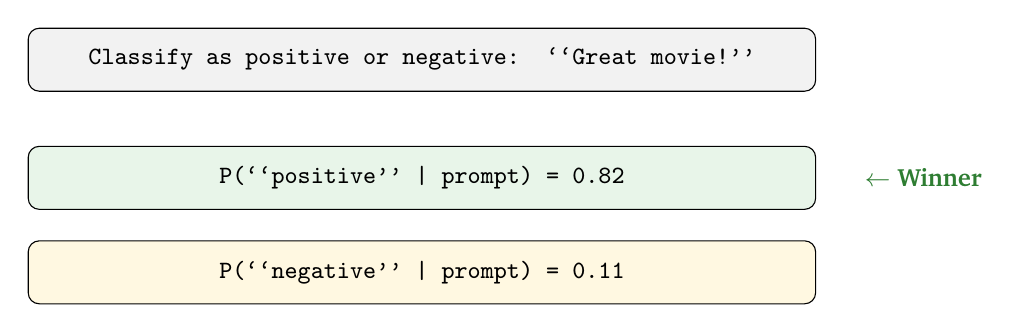
\begin{tikzpicture}[
    box/.style={draw, rounded corners, fill=#1, minimum width=10cm, minimum height=0.8cm, align=left, font=\small\ttfamily},
    arrow/.style={-{Stealth[length=2mm]}, thick, color=accent}
]
\node[box=gray!10] (prompt) at (0, 0) {Classify as positive or negative: ``Great movie!''};
\node[box=tipbg] (pos) at (0, -1.5) {P(``positive'' | prompt) = 0.82};
\node[box=warnbg] (neg) at (0, -2.7) {P(``negative'' | prompt) = 0.11};
\node[font=\small\bfseries\color{codegreen}, right] at (5.5, -1.5) {$\leftarrow$ Winner};
\end{tikzpicture}
\caption{Logprob classification. Instead of generating text, we directly compare the probability the model assigns to each label. This eliminates parsing ambiguity entirely.}
\label{fig:logprob}
\end{figure}

\textbf{Why this is better than generation:} There is no text to parse. The model either assigns higher probability to the correct label or it does not. No formatting ambiguity, no partial matches, no prompt sensitivity.

\textbf{Limitations:} It only works for classification tasks where you can define a small set of possible labels. You cannot use this method for open-ended generation tasks.

\textbf{Our setup:} 200 examples per language, balanced 50/50 positive/negative. Chance performance = 50\%.

\subsubsection{Method 2: Generative Classification}

\textbf{What it measures:} Can the model follow an instruction and produce a correctly formatted answer?

\textbf{How it works:} Give the model a prompt like ``Classify this text as positive or negative'' and let it generate a free-form response. Then parse the response for sentiment labels.

\textbf{Why include this:} This is closer to how real users interact with models. A model that ``knows'' the answer (high logprob) but cannot \emph{express} it (fails generative) has a practical limitation.

\textbf{Limitations:} Fragile. The model might understand the task perfectly but produce output like ``I think the sentiment is mostly positive with some caveats'' which fails a strict parser. We mitigate this by accepting multiple formats (``positive,'' ``Positive,'' ``pos,'' etc.).

\textbf{Our setup:} 50 examples per language, balanced 50/50. Chance performance = 0\% (the model must produce a parseable label; random text will not match).

\subsubsection{Method 3: Cross-Lingual Retrieval}

\textbf{What it measures:} Does the model understand that the same meaning in different languages should have similar internal representations?

\textbf{How it works:}
\begin{enumerate}
    \item Take a sentence in language A (e.g., English).
    \item Take 10 sentences in language B (e.g., Hebrew)---one is the correct translation, nine are random distractors.
    \item Feed all 11 sentences through the model and extract their \textbf{embeddings} (internal vector representations) from the last hidden layer.
    \item Measure which of the 10 Hebrew sentences has the most similar embedding to the English sentence (using cosine similarity).
    \item If the correct translation is most similar, count it as a hit.
\end{enumerate}

\begin{figure}[H]
\centering
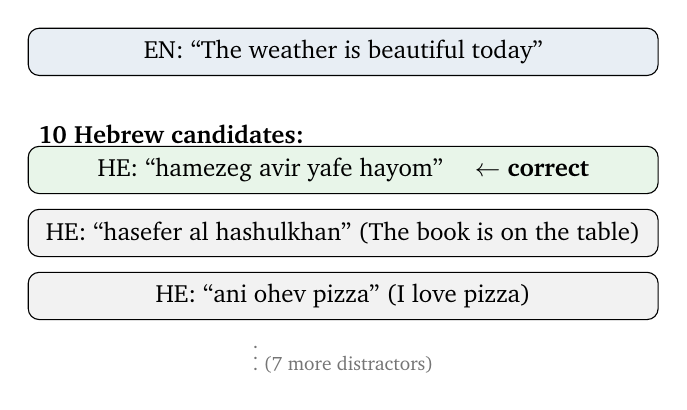
\begin{tikzpicture}[
    sent/.style={draw, rounded corners, fill=#1, minimum width=8cm, minimum height=0.6cm, align=left, font=\small},
]
\node[sent=lightaccent] (en) at (0, 0) {EN: ``The weather is beautiful today''};
\node[font=\small\bfseries, below=0.5cm of en, anchor=north west, xshift=-4cm] {10 Hebrew candidates:};
\node[sent=tipbg] (he1) at (0, -1.5) {HE: ``hamezeg avir yafe hayom'' \quad\textbf{$\leftarrow$ correct}};
\node[sent=gray!10] (he2) at (0, -2.3) {HE: ``hasefer al hashulkhan'' (The book is on the table)};
\node[sent=gray!10] (he3) at (0, -3.1) {HE: ``ani ohev pizza'' (I love pizza)};
\node[font=\scriptsize\color{codegray}] at (0, -3.8) {$\vdots$ (7 more distractors)};
\end{tikzpicture}
\caption{Cross-lingual retrieval. The model must identify the correct translation from 10 candidates using only its internal representations. Chance = 10\%.}
\label{fig:retrieval}
\end{figure}

\textbf{Why this matters:} Retrieval accuracy measures the quality of the model's \emph{internal representations}, not its generation ability. High retrieval accuracy means the model has learned that the same concept in different languages should ``look similar'' internally. This is the foundation of cross-lingual transfer.

\textbf{Our setup:} 10-way retrieval for all language pairs. Chance = 10\%.

\subsubsection{Additional Evaluation: Belebele Reading Comprehension}

\textbf{Belebele} \citep{bandarkar2023belebele} is a standardized reading comprehension benchmark available in 122 languages. Each question gives a passage and four answer choices. We include it to test whether our model can perform abstract reasoning, not just classification.

Spoiler: at 3B scale, it cannot. All results are near the 25\% chance level. This is expected and honest---it tells us where our model's capabilities end.

\subsection{Evaluation Set Construction}

The quality of your evaluation sets is as important as the quality of your training data. Here are the rules we follow:

\begin{enumerate}
    \item \textbf{Balance all classes.} Every evaluation set has exactly 50\% positive and 50\% negative examples (for binary classification). This makes chance performance exactly 50\%, which is a clean baseline.
    
    \item \textbf{Sufficient size.} We use 200 examples per language for logprob (statistical power for detecting $>$5pp differences) and 50 for generative (slower to run).
    
    \item \textbf{Native-language sources.} Each language's evaluation data comes from a \emph{native} dataset in that language---not translations from English. This ensures we are testing real-world text, not translation artifacts.
    
    \item \textbf{Strict separation.} Evaluation examples are held out before any training begins. They are never seen during pretraining or SFT.
    
    \item \textbf{Shuffled sampling.} We shuffle the source dataset before selecting evaluation examples, ensuring a random distribution of topics, authors, and styles.
\end{enumerate}

\begin{warning}
We cannot stress this enough: \textbf{verify your evaluation sets manually.} In our early experiments, we discovered that 31.4\% of our Hebrew evaluation labels were wrong (due to a label inversion bug), and our Arabic evaluation set contained only negative examples (due to a sorting artifact). Both bugs produced results that looked plausible---they just happened to be completely wrong. See Chapter~\ref{ch:lessons} for details.
\end{warning}

\subsection{Interpreting Results: What Counts as ``Good''?}

When you see that your model gets 84.5\% on Hebrew sentiment, is that good? Context matters:

\begin{table}[H]
\centering
\begin{tabular}{ll}
\toprule
\textbf{Benchmark} & \textbf{What counts as good} \\
\midrule
Logprob sentiment (chance=50\%) & 70\%+ is meaningful; 85\%+ is strong \\
Generative sentiment (chance=0\%) & 50\%+ shows task understanding; 80\%+ is strong \\
Cross-lingual retrieval (chance=10\%) & 50\%+ is meaningful; 80\%+ is strong \\
Belebele (chance=25\%) & 40\%+ at 3B would be notable \\
\bottomrule
\end{tabular}
\caption{Rough interpretation guide. These thresholds are specific to our model size (3B) and evaluation setup.}
\label{tab:interpretation}
\end{table}

Comparing against larger models is useful for context but not the primary goal. Our research questions are about \emph{relative} performance: does multilingual SFT beat English-only SFT? Does the tokenizer affect efficiency? These comparisons use the same model and same evaluation, making them internally valid regardless of absolute performance.

\begin{reporef}
\textbf{Evaluation scripts:}\hfill\texttt{eval/scripts/}\\
\quad\texttt{exp\_a\_fix\_classification.py}\hfill Sentiment classification (logprob + generative)\\
\quad\texttt{exp\_b\_crosslingual.py}\hfill Cross-lingual BPB evaluation\\
\quad\texttt{eval\_embeddings.py}\hfill Cross-lingual retrieval\\
\quad\texttt{eval\_belebele.py}\hfill Belebele reading comprehension\\
\quad\texttt{exp\_c\_tokenizer\_ablation.py}\hfill Tokenizer efficiency comparison\\
\quad\texttt{tokenizer\_analysis.py}\hfill Detailed tokenizer metrics\\
[4pt]
\textbf{Evaluation results:}\hfill\texttt{eval/results/}\\
\quad\texttt{v4\_results.json}\hfill Final v4 results (post-data-fix)\\
\quad\texttt{exp\_a\_fix\_results.json}\hfill Experiment A sentiment results\\
\quad\texttt{exp\_ab\_results.json}\hfill Combined A+B results\\
\quad\texttt{exp\_c\_tokenizer\_ablation.json}\hfill Tokenizer comparison data\\
\quad\texttt{belebele\_3b\_results.json}\hfill Belebele benchmark results\\
[4pt]
\textbf{Evaluation prompts:}\hfill\texttt{eval/prompts/prompts.md}\\
\end{reporef}

\subsection{Summary: Evaluation Principles}

\begin{enumerate}
    \item \textbf{Use multiple evaluation methods.} No single metric tells the whole story. Logprob measures knowledge; generative measures usability; retrieval measures representations.
    \item \textbf{Balance your evaluation sets.} Unbalanced sets hide model weaknesses.
    \item \textbf{Use native-language data.} Translated evaluation data introduces artifacts.
    \item \textbf{Verify labels manually.} Spot-check at least 50 examples per language.
    \item \textbf{Report chance baselines.} Always state what random performance would be, so readers can judge whether your results are meaningful.
    \item \textbf{Include negative results.} Report tasks where your model fails (like our Belebele results). This is honest and informative.
\end{enumerate}

\begin{tip}
Build your evaluation pipeline \emph{before} you start training, and run it on the base model first. The base model results establish your baseline and verify that the evaluation code works correctly. If your base model gets 95\% accuracy on a balanced binary task, something is wrong with your evaluation, not right with your model.
\end{tip}

\begin{successcheck}
\begin{itemize}[nosep]
  \item Base model results are near chance level (confirms evaluation is not leaking)
  \item Multilingual SFT model outperforms base on all languages and methods
  \item Results are consistent across evaluation methods (logprob and generative agree directionally)
  \item Evaluation sets are exactly balanced (50/50 for binary tasks)
  \item All results are saved as raw outputs, not just summary statistics
\end{itemize}
\end{successcheck}

\begin{failuresign}
\begin{itemize}[nosep]
  \item Base model scores well above chance --- data leakage or evaluation bug
  \item 100\% accuracy on any task --- single-class evaluation set or memorization
  \item Logprob and generative results disagree strongly --- prompt format may be wrong for one method
  \item Results vary wildly between runs --- evaluation set is too small (increase N)
\end{itemize}
\end{failuresign}

% ============================================================
% CHAPTER 9: PLACEHOLDER
% ============================================================

\section{Results: What SemiticGPT Can Do}
\label{ch:results}

\begin{center}
\colorbox{lightaccent}{\textbf{Track: Concept}}
\end{center}

This chapter presents our experimental results. We organize them around three questions, each addressed by a dedicated experiment.

\subsection{Experiment A: Does Multilingual SFT Work?}

The most basic question: after pretraining and multilingual fine-tuning, can the model actually classify sentiment across all four languages?

\begin{table}[H]
\centering
\begin{tabular}{lccccc}
\toprule
\textbf{Stage} & \textbf{HE} & \textbf{AR} & \textbf{FA} & \textbf{EN} \\
\midrule
\multicolumn{5}{l}{\textit{Logprob classification (N=200, chance=50\%)}} \\
Base (pretrained only) & 53.0 & 45.0 & 60.5 & 51.5 \\
EN-SFT (English only) & 51.5 & 46.5 & 58.5 & 52.0 \\
Multi-SFT & \textbf{84.5} & \textbf{60.5} & \textbf{78.5} & \textbf{73.0} \\
\midrule
\multicolumn{5}{l}{\textit{Generative classification (N=50, chance=0\%)}} \\
Base & 0 & 0 & 0 & 0 \\
EN-SFT & 0 & 0 & 0 & 2 \\
Multi-SFT & \textbf{82} & \textbf{64} & \textbf{74} & \textbf{64} \\
\bottomrule
\end{tabular}
\caption{Sentiment classification accuracy (\%) across three model stages. The three-stage comparison separates what the model learns from pretraining alone, from English-only task training, and from multilingual task training.}
\label{tab:results_sentiment}
\end{table}

\textbf{How to read this table:}

\begin{itemize}
    \item \textbf{Base model} (row 1): Near chance (50\%) for logprob, zero for generative. The pretrained model has no task-following ability. It ``knows'' these languages but cannot use that knowledge for classification.
    
    \item \textbf{EN-SFT} (row 2): Almost no improvement. Training on English-only examples does not help the model classify sentiment in \emph{any} language, including English itself. This is the key negative result.
    
    \item \textbf{Multi-SFT} (row 3): Large gains everywhere. Hebrew improves by 31.5 percentage points (logprob), Arabic by 15.5pp, Persian by 18pp, English by 21.5pp.
\end{itemize}

\begin{figure}[H]
\centering
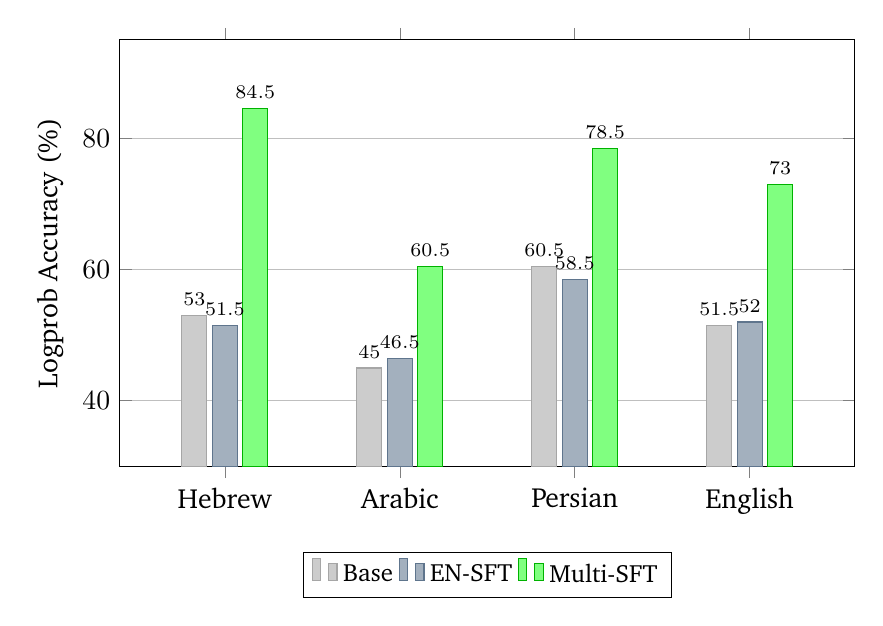
\begin{tikzpicture}
\begin{axis}[
    ybar,
    bar width=9pt,
    ylabel={Logprob Accuracy (\%)},
    symbolic x coords={Hebrew, Arabic, Persian, English},
    xtick=data,
    ymin=30, ymax=95,
    legend style={at={(0.5,-0.2)}, anchor=north, legend columns=3, font=\small},
    nodes near coords,
    nodes near coords align={vertical},
    every node near coord/.append style={font=\scriptsize},
    width=0.9\textwidth,
    height=7cm,
    ymajorgrids=true,
    enlarge x limits=0.2,
]
\addplot[fill=gray!40, draw=gray!70] coordinates {(Hebrew,53.0) (Arabic,45.0) (Persian,60.5) (English,51.5)};
\addplot[fill=accent!40, draw=accent!70] coordinates {(Hebrew,51.5) (Arabic,46.5) (Persian,58.5) (English,52.0)};
\addplot[fill=green!50, draw=green!70!black] coordinates {(Hebrew,84.5) (Arabic,60.5) (Persian,78.5) (English,73.0)};
\legend{Base, EN-SFT, Multi-SFT}
\end{axis}
\end{tikzpicture}
\caption{The visual story: the gray bars (base) and blue bars (EN-SFT) are nearly identical, meaning English-only fine-tuning does almost nothing. The green bars (Multi-SFT) show substantial improvement across all languages.}
\label{fig:results_sentiment}
\end{figure}

\begin{keyidea}
The central finding: at 3B scale with 4.48B pretraining tokens, \textbf{English-only SFT is insufficient for cross-lingual task transfer}. The model needs explicit examples in each target language to perform downstream tasks. Multilingual pretraining creates shared representations, but those representations cannot be activated for tasks without multilingual fine-tuning.
\end{keyidea}

\begin{tip}[title={Builder Takeaway}]
Do not assume English-only SFT will transfer. Budget time and data for multilingual fine-tuning from the start. Even small amounts of native-language SFT data (a few thousand examples per language) produce large gains.
\end{tip}

\subsection{Experiment B: Cross-Lingual Transfer Analysis}

Experiment A showed that multilingual SFT works. Experiment B asks \emph{why} English-only SFT does not, and what the pretrained model \emph{has} learned about cross-lingual structure.

\subsubsection{The Pretrained Model Has Cross-Lingual Representations}

Despite the EN-SFT failure, the base model develops strong cross-lingual alignment purely from pretraining:

\begin{table}[H]
\centering
\begin{tabular}{lcc}
\toprule
\textbf{Direction} & \textbf{Base} & \textbf{Multi-SFT} \\
\midrule
EN$\rightarrow$HE & \textbf{90\%} & 90\% \\
HE$\rightarrow$EN & \textbf{90\%} & 80\% \\
AR$\rightarrow$EN & 70\% & 50\% \\
AR$\rightarrow$HE & 70\% & 70\% \\
EN$\rightarrow$AR & 50\% & 60\% \\
HE$\rightarrow$AR & 40\% & 60\% \\
FA$\rightarrow$HE & 50\% & 30\% \\
HE$\rightarrow$FA & 40\% & 30\% \\
EN$\rightarrow$FA & 20\% & 20\% \\
AR$\rightarrow$FA & 10\% & 10\% \\
FA$\rightarrow$EN & 10\% & 10\% \\
FA$\rightarrow$AR & 10\% & 10\% \\
\midrule
\textbf{Average} & \textbf{45.8\%} & \textbf{43.3\%} \\
\bottomrule
\end{tabular}
\caption{Cross-lingual retrieval accuracy (10-way, chance=10\%). English$\leftrightarrow$Hebrew retrieval reaches 90\%---9$\times$ chance---purely from pretraining.}
\label{tab:results_retrieval}
\end{table}

This is a striking result: the model places English and Hebrew sentences with the same meaning very close together in its internal representation space, even though it was never explicitly trained to do so. Cross-lingual alignment \emph{emerged} from the simple task of predicting the next token across multilingual data.

\subsubsection{A Language Family Hierarchy}

The retrieval results reveal a clear hierarchy of cross-lingual connectivity:

\begin{enumerate}
    \item \textbf{English $\leftrightarrow$ Hebrew: 90\%} --- Strongest pair. Hebrew is the anchor language (40\% of data) and English is the bridge language. Both are well-represented.
    \item \textbf{Arabic $\leftrightarrow$ English/Hebrew: 40--70\%} --- Moderate connectivity. Arabic shares Semitic roots with Hebrew, which helps.
    \item \textbf{Persian $\leftrightarrow$ everything: 10--50\%} --- Weak connectivity. Despite sharing Arabic script, Persian is typologically distant (Indo-European, not Semitic).
\end{enumerate}

This pattern is consistent with \textbf{linguistic family membership being a stronger predictor of cross-lingual transfer than script similarity}. Arabic script does not automatically create alignment between Arabic and Persian; shared Semitic grammar creates alignment between Arabic and Hebrew.

\subsubsection{The Representation--Task Gap}

Here is the puzzle: the base model achieves 90\% EN$\leftrightarrow$HE retrieval (strong representations) but only 53\% Hebrew sentiment accuracy (near chance). How can it ``know'' these languages are related but be unable to use that knowledge?

The answer is that \textbf{representation alignment} and \textbf{task transfer} are different capabilities:

\begin{itemize}
    \item \textbf{Representation alignment} means the model's internal vectors for similar concepts are close together across languages. This emerges naturally from multilingual pretraining.
    \item \textbf{Task transfer} means the model can apply a learned behavior (like sentiment classification) across languages. This requires explicit instruction.
\end{itemize}

An analogy: imagine you have a detailed multilingual map (representation alignment). You can see that Tel Aviv and Paris are both cities. But knowing they are both cities does not tell you how to navigate from one to the other---you need explicit directions (task transfer via SFT).

\subsubsection{The Retrieval--SFT Trade-off}

An interesting secondary finding: after multilingual SFT, average retrieval accuracy drops slightly (45.8\% $\rightarrow$ 43.3\%). Fine-tuning makes the model better at classification but slightly worse as a general-purpose cross-lingual encoder. This is a common phenomenon: optimizing for one capability can come at a small cost to another. The model's internal representations become more task-focused and slightly less general-purpose.

\begin{tip}[title={Builder Takeaway}]
Your pretrained model already learns cross-lingual structure---you do not need to engineer it explicitly. Linguistic family membership predicts transfer better than script similarity. When choosing languages, prioritize related language families over shared scripts.
\end{tip}

\subsection{Experiment C: Tokenizer Efficiency}

Experiment C is purely about the tokenizer---no model training required. We compare our custom tokenizer against Llama-2 (English-centric) and HebrewGPT (Hebrew-centric), all with 32K vocabularies.

The detailed results were presented in Chapter~\ref{ch:tokenizer}. The headline numbers:

\begin{itemize}
    \item \textbf{Hebrew}: 66\% fewer tokens than Llama-2 (1.34 vs 3.91 tokens/word)
    \item \textbf{Arabic}: 49\% fewer tokens (2.22 vs 4.36)
    \item \textbf{Persian}: 69\% fewer tokens (1.52 vs 4.88)
    \item \textbf{English}: 2\% \emph{more} tokens (1.54 vs 1.51)---negligible penalty
\end{itemize}

In practical terms: for every Hebrew document, our model processes 3$\times$ more text in the same context window compared to using Llama-2's tokenizer. For Persian, it is 3.2$\times$ more. This is a massive efficiency gain that costs almost nothing on English.

\begin{tip}[title={Builder Takeaway}]
Never reuse an English-centric tokenizer for non-Latin languages. The 2--3 day investment in building a custom tokenizer pays for itself immediately: 3$\times$ more text per context window means 3$\times$ more efficient training and inference.
\end{tip}

\subsection{Belebele: Where the Model Fails}

Belebele reading comprehension results are near chance (25\%) for all stages and all languages:

\begin{table}[H]
\centering
\begin{tabular}{lcccc}
\toprule
\textbf{Stage} & \textbf{HE} & \textbf{AR} & \textbf{FA} & \textbf{EN} \\
\midrule
Random & 25.0 & 25.0 & 25.0 & 25.0 \\
Base & 26.0 & 22.0 & 19.0 & 19.0 \\
Multi-SFT & 28.0 & 24.0 & 25.0 & 23.0 \\
\bottomrule
\end{tabular}
\caption{Belebele reading comprehension (\%, 4-way multiple choice, N=100). All near chance (25\%).}
\label{tab:results_belebele}
\end{table}

This is expected: Belebele requires reading a passage, understanding a question, and selecting the correct answer from four choices. This level of abstract reasoning typically requires models of 7B+ parameters with much larger pretraining corpora. We include these results because \textbf{reporting where your model fails is as important as reporting where it succeeds}. It tells practitioners what tasks are out of reach at this scale.

\begin{tip}[title={Builder Takeaway}]
Know your model's ceiling. At 3B parameters, expect strong classification and retrieval but near-chance reading comprehension. If you need reasoning capabilities, plan for 7B+ from the start---or scope your evaluation to tasks that match your scale.
\end{tip}

\subsection{Summary of Results}

\begin{table}[H]
\centering
\begin{tabular}{lp{10cm}}
\toprule
\textbf{Finding} & \textbf{Significance} \\
\midrule
Multilingual SFT required & English-only fine-tuning does not transfer to other languages at 3B scale. Each language needs its own task examples. \\
Cross-lingual representations emerge & The base model learns that related languages belong in a shared semantic space, purely from next-token prediction. \\
Representation $\neq$ task transfer & Good cross-lingual embeddings do not automatically enable cross-lingual task performance. \\
Anchor language benefits & Hebrew (40\% data share) achieves the strongest results across all experiments. \\
Family $>$ script & Persian shares Arabic script but shows weak transfer. Hebrew--Arabic transfer is stronger, consistent with shared Semitic grammar. \\
Tokenizer efficiency is critical & 49--69\% fewer tokens for target languages with minimal English penalty. \\
Scale limitations are real & 3B is insufficient for reading comprehension (Belebele near chance). \\
\bottomrule
\end{tabular}
\caption{Summary of experimental findings and their practical implications.}
\end{table}

\begin{tip}[title={Builder Takeaway}]
The most actionable findings: (1) build a custom tokenizer---it is a 2-day investment with 3$\times$ efficiency gains, (2) include multilingual SFT data from day one---English-only does not transfer at 3B scale, (3) set expectations by scale---sentiment classification yes, reading comprehension no.
\end{tip}


% ============================================================
% CHAPTER 10: WHAT WENT WRONG
% ============================================================

\section{What Went Wrong: Data Bugs, Failed Runs, and Hard Lessons}
\label{ch:lessons}

\begin{center}
\colorbox{lightaccent}{\textbf{Track: Concept + Build}}
\end{center}

\begin{warning}[title={Read This Before Your First Training Run}]
This chapter describes eight real failures that cost us days of compute and weeks of debugging. Every single one could have been prevented with a 10-minute verification check. If you are about to launch your first training run, read at least Lessons~1--3 (label inversion, sorting artifacts, data leakage) and the Verification Checklist at the end. These three bugs account for the majority of beginner failures.
\end{warning}

This may be the most valuable chapter in the guide. Every published paper shows polished results; very few show the failures that preceded them. Our path to working results included inverted labels, contaminated evaluation, sorting artifacts, crashed training runs, and wasted compute. Each mistake taught us something useful.

\subsection{Lesson 1: The Hebrew Label Inversion}

\textbf{What happened:} Our Hebrew sentiment dataset (\texttt{mteb/hebrew\_sentiment\_analysis}) encodes labels as integers: 0 = positive, 1 = negative, 2 = off-topic. Our data preparation script assumed the standard convention: 0 = negative, 1 = positive. Every Hebrew label was flipped.

\textbf{How we discovered it:} We achieved 80\% accuracy on Hebrew sentiment, which seemed excellent. But when we manually inspected the predictions, the model was calling clearly negative tweets ``positive'' and vice versa. A keyword-based audit (checking for positive words in ``negative'' predictions) confirmed that 31.4\% of labels were inconsistent.

\textbf{The real damage:} The 80\% accuracy was measuring how well the model learned the \emph{wrong} mapping. It was not a sign of capability---it was a sign that the model was faithfully learning incorrect labels.

\textbf{The fix:} Read the dataset's documentation. Check the \texttt{ClassLabel} object: \texttt{names=['pos', 'neg', 'off-topic']}, meaning index 0 = positive, index 1 = negative. Our script now explicitly maps from the dataset's schema rather than assuming a convention.

\begin{warning}
\textbf{Different datasets encode the same concept differently.} SST-2 uses 0=negative, 1=positive. Hebrew Sentiment uses 0=positive, 1=negative. There is no universal standard. \textbf{Always read the dataset card} and verify with manual inspection.
\end{warning}

\subsection{Lesson 2: The Arabic Sorting Artifact}

\textbf{What happened:} Our Arabic sentiment dataset (\texttt{arbml/Sentiment\_Analysis\_Tweets}) was sorted by label in the source data: all 29,100 negative tweets first, then all 38,970 positive tweets. Our script loaded the first 10,000 examples for training and the next 500 for evaluation.

Result: both training and evaluation sets contained \textbf{only negative examples}.

\textbf{How we discovered it:} The model achieved 100\% accuracy on Arabic sentiment. This was suspicious---no model gets 100\% on a real task. A simple \texttt{value\_counts()} on the labels confirmed: zero positive examples in either set.

\textbf{The real damage:} 100\% accuracy on a test with only one class is trivially achieved by always predicting that class. The metric was meaningless.

\textbf{The fix:} \textbf{Always shuffle before splitting.} Our data preparation script now enforces: (1) load the full dataset, (2) shuffle with a fixed random seed, (3) \emph{then} split into train/eval. Additionally, we verify that both classes are present in both splits.

\begin{tip}
Add a simple assertion to your data pipeline:
\begin{lstlisting}[language=Python]
assert len(set(eval_labels)) >= 2, \
    f"Eval set has only {set(eval_labels)} classes!"
assert abs(eval_labels.mean() - 0.5) < 0.1, \
    f"Eval set imbalanced: {eval_labels.mean():.1%} positive"
\end{lstlisting}
These two lines would have caught our Arabic bug immediately.
\end{tip}

\subsection{Lesson 3: Data Leakage}

\textbf{What happened:} Our v3 training script accidentally included the evaluation files in the training data. The model was tested on examples it had already memorized.

\textbf{How we discovered it:} When we ran the same evaluation on a freshly prepared dataset (v4, with strict separation), results dropped significantly. The v3 ``good results'' were partially memorization.

\textbf{The fix:} Strict file-level separation. Evaluation data is prepared in a separate script, saved to separate files, and never loaded by the training script. We verify separation by checking that no example in the evaluation set appears in the training set (using exact string matching).

\begin{keyidea}
Data leakage is insidious because \textbf{it produces results that look correct}. The model genuinely gets the right answer---it just does so by remembering, not understanding. The only reliable defense is strict process: separate data pipelines for training and evaluation, with automated verification.
\end{keyidea}

\subsection{Lesson 4: Translation Data Quality}

\textbf{What happened:} Our v3 translation training data was supposed to contain thousands of real sentence pairs from OPUS-100. Instead, the download URLs had changed (404 errors), and the fallback code silently used 50 hardcoded example pairs. The model's translation ``training'' consisted of memorizing 50 sentences.

\textbf{How we discovered it:} By checking the actual file sizes. The translation training file was 4 KB instead of the expected 400 KB.

\textbf{The fix:} For v4, we download directly from HuggingFace's datasets library (\texttt{Helsinki-NLP/opus-100}), which provides stable access. We also added size checks: if a downloaded dataset has fewer than 1,000 examples, the script raises an error rather than silently proceeding.

\subsection{Lesson 5: The Failed 1B Training Run}

\textbf{What happened:} Before the successful 3B run, we attempted a 1B parameter model. The training used a cosine schedule with 3 warm restarts over 15,000 steps. The model peaked at step 2,000 (about 1B tokens seen), then validation loss \emph{increased} continuously through step 4,500, at which point we terminated.

\textbf{Root cause:} The cosine schedule with warm restarts decayed the learning rate too aggressively. By step 4,000, the learning rate had dropped to near zero, with 73\% of training steps remaining at an ineffective learning rate. The warm restarts briefly increased LR but not enough to recover.

\textbf{What we learned:} This failure directly motivated the proxy experiments (Chapter~\ref{ch:proxy}). We tested the fix at 110M scale first, confirmed that a simple cosine schedule (no restarts) with AdamW worked correctly, and only then committed to the 3B run. The 3B run completed successfully with monotonically decreasing loss---40 consecutive new bests, zero plateau.

\subsection{Lesson 6: Optimizer Instability}

\textbf{What happened:} Our proxy experiments initially used the Muon optimizer, which had shown promising results in other contexts. At learning rates above 0.02, Muon caused training loss to explode (validation BPB jumped from $\sim$15 to $\sim$700). Three of eight Muon experiments diverged.

\textbf{What we learned:} Newer, more exotic optimizers may offer advantages but also carry risks. AdamW is ``boring'' but reliable---it never diverged in any of our 24 AdamW experiments. For a project where you have one shot at a multi-day training run, reliability matters more than marginal convergence speed.

\subsection{Lesson 7: Architecture Mismatch}

\textbf{What happened:} Our v2 SFT evaluation loaded the model using a simplified transformer class instead of the actual GPT architecture used during pretraining. The simplified class lacked fused QKV projections and RoPE position encoding. The model weights loaded without errors (the parameter names happened to match) but the computation was wrong.

\textbf{How we discovered it:} v2 results were mediocre despite ``identical'' training. A code review revealed the architecture class mismatch.

\textbf{The fix:} Use exactly the same model class for training, SFT, and evaluation. Define the architecture once and import it everywhere. Never copy-paste model code between scripts.

\subsection{The Meta-Lesson}

\begin{keyidea}
Every mistake in this chapter has the same structure:
\begin{enumerate}
    \item Something \emph{appeared} to work.
    \item We did not verify the assumption.
    \item Later discovery invalidated the results.
\end{enumerate}

The defense is systematic verification at every stage: check your labels, check your data splits, check your model architecture, check your file sizes. The 10 minutes you spend verifying will save you days of wasted training.
\end{keyidea}

\subsection{Verification Checklist}

Here is the checklist we now run before every training job:

\begin{enumerate}
    \item[$\square$] \textbf{Labels:} Manually inspect 20+ examples per language. Do the labels match the text?
    \item[$\square$] \textbf{Balance:} Run \texttt{value\_counts()} on labels for both train and eval sets.
    \item[$\square$] \textbf{Separation:} Verify zero overlap between train and eval examples.
    \item[$\square$] \textbf{Data size:} Check file sizes. Are they in the expected range?
    \item[$\square$] \textbf{Architecture:} Verify the same model class is used for training and evaluation.
    \item[$\square$] \textbf{Baseline:} Run evaluation on the base model. Are results near chance?
    \item[$\square$] \textbf{Instance:} Verify GPU type and training speed in the first 30 minutes.
    \item[$\square$] \textbf{Checkpointing:} Verify that checkpoint saving and loading works before starting a long run.
\end{enumerate}

% ============================================================
% CHAPTER 11: PLACEHOLDER
% ============================================================

\section{Practitioner's Checklist: Building Your Own Multilingual Model}
\label{ch:checklist}

\begin{center}
\colorbox{tipbg}{\textbf{Track: Build}}
\end{center}

This final chapter distills the entire guide into a step-by-step recipe. If you are building a multilingual language model for your own language cluster, this is your roadmap. Each step references the relevant chapter for deeper explanation and the relevant repository artifact for code.

\subsection{Smallest Viable Version}

If this is your first model, start small. The table below shows three build scales---\textbf{start with Toy} to verify your pipeline end-to-end, then scale up.

\begin{table}[H]
\centering
\begin{tabular}{lccc}
\toprule
& \textbf{Toy} & \textbf{Practical} & \textbf{Full} \\
\midrule
Languages & 2 & 3--4 & 4--6 \\
Parameters & 100--300M & 1--3B & 3--7B \\
Training tokens & 50--200M & 1--5B & 5--20B \\
GPUs & 1 & 1--4 & 4--8 \\
Task & Sentiment only & Sentiment + translation & Multiple tasks \\
Evaluation & Logprob only & Logprob + generative & Full suite \\
Time (end-to-end) & 1--3 days & 1--2 weeks & 3--5 weeks \\
Cost & \$10--50 & \$200--1,000 & \$1,000--5,000 \\
\bottomrule
\end{tabular}
\caption{Three build scales. Start with Toy to validate your pipeline, then scale.}
\end{table}

\textbf{The Toy build:}
\begin{itemize}[nosep]
  \item \textbf{2 languages} --- your anchor language + English.
  \item \textbf{100--300M parameters} --- trains in minutes on 1 GPU.
  \item \textbf{50--200M tokens} --- enough to see learning curves.
  \item \textbf{Sentiment classification only} --- the simplest end-to-end task.
  \item \textbf{Logprob evaluation only} --- fast, deterministic, no generation needed.
\end{itemize}

The purpose of the Toy build is \textbf{not} to get good results. It is to verify that every component of your pipeline works: tokenizer $\rightarrow$ data loading $\rightarrow$ training loop $\rightarrow$ checkpointing $\rightarrow$ SFT $\rightarrow$ evaluation. If any step is broken, you will discover it in hours instead of days.

\begin{tip}
Our proxy experiments (Chapter~\ref{ch:proxy}) are effectively the Toy build. The 110M proxy used the same code, data, and tokenizer as the full 3B run. Start there.
\end{tip}

\subsection{Phase 1: Define Your Scope (1--2 days)}

Before writing any code, answer these questions:

\begin{table}[H]
\centering
\begin{tabular}{lp{8cm}l}
\toprule
\textbf{Question} & \textbf{Our Answer} & \textbf{Chapter} \\
\midrule
Which languages? & Hebrew, Arabic, Persian, English & \ref{ch:what_is_lm} \\
Why these languages? & Semitic family cluster + Persian as control & \ref{ch:what_is_lm} \\
What tasks? & Sentiment classification, cross-lingual transfer & \ref{ch:eval} \\
What model size? & 3B (fits one GPU for inference, trainable on one node) & \ref{ch:architecture} \\
What hardware? & 8$\times$H100 (p5en.48xlarge) for pretraining; 1$\times$A10G for SFT & \ref{ch:pretraining} \\
What is the anchor language? & Hebrew (40\% of pretraining data) & \ref{ch:data} \\
\bottomrule
\end{tabular}
\caption{Scoping questions. Answer these before starting.}
\end{table}

\begin{tip}
Choose your languages based on a \textbf{linguistic hypothesis}, not just convenience. We chose Hebrew + Arabic (Semitic siblings) + Persian (same script, different family) + English (bridge) specifically to test whether linguistic relatedness predicts transfer better than script similarity.
\end{tip}

\subsection{Phase 2: Build the Tokenizer (1--2 days)}

\begin{enumerate}
    \item \textbf{Collect balanced text samples.} Equal proportion from each target language. 100MB--1GB per language is sufficient for tokenizer training.
    
    \item \textbf{Train SentencePiece BPE.} Use 32K vocabulary for 4--6 languages (64K if more). Enable byte fallback and NFKC normalization.
    
    \item \textbf{Add special tokens.} Define \texttt{<s>}, \texttt{</s>}, \texttt{<pad>}, and any instruction tokens (\texttt{<|user|>}, \texttt{<|assistant|>}) before training.
    
    \item \textbf{Verify fertility.} Compute tokens-per-word on held-out text for each language. Target: $\leq$2.0 for all languages. Check that English penalty is $<$5\%.
    
    \item \textbf{Inspect vocabulary composition.} Check the script distribution in the vocabulary. It should roughly reflect your language mix.
\end{enumerate}

\begin{reporef}
\textbf{Script:} \texttt{tokenizer/scripts/train\_tokenizer.py}\hfill
\textbf{Config:} \texttt{tokenizer/config/tokenizer\_config.json}\hfill
\textbf{Output:} \texttt{tokenizer/artifacts/}
\end{reporef}

\subsection{Phase 3: Collect and Prepare Data (1--2 weeks)}

This is the most time-consuming phase. Do not rush it.

\begin{enumerate}
    \item \textbf{Identify sources.} For each language: Wikipedia, OSCAR/Common Crawl, news corpora, government documents, domain-specific text.
    
    \item \textbf{Download and deduplicate.} Use MinHash deduplication to remove near-duplicates.
    
    \item \textbf{Filter for quality.} Run language identification to remove mislabeled documents. Apply perplexity-based filtering using a small reference model.
    
    \item \textbf{Tokenize.} Convert clean text to token IDs using your custom tokenizer. Store as uint16 binary files.
    
    \item \textbf{Mix to target proportions.} Combine language-specific files according to your target distribution (e.g., 40/20/20/20).
    
    \item \textbf{Create manifests.} Record every source, its license, size, and processing steps. You will need this for reproducibility and debugging.
    
    \item \textbf{Verify.} Spot-check 100+ decoded examples per language. Do they look like clean, natural text in the expected language?
\end{enumerate}

\begin{reporef}
\textbf{Collection scripts:} \texttt{data/scripts/}\hfill
\textbf{Manifests:} \texttt{data/manifests/}
\end{reporef}

\subsection{Phase 4: Run Proxy Experiments (2--3 days)}

\begin{enumerate}
    \item \textbf{Define a proxy model.} Scale down your architecture by $\sim$25--30$\times$. Our 3B model scaled down to 110M for proxies.
    
    \item \textbf{Write the experiment program.} List what you want to test, in priority order: LR schedule, optimizer, peak LR, training duration, weight decay, regularization.
    
    \item \textbf{Run 20--40 experiments.} Each should take 2--10 minutes. Use the same data and tokenizer as the full run.
    
    \item \textbf{Select the winner.} Choose the configuration with the best validation BPB, breaking ties by simplicity and stability.
    
    \item \textbf{Document everything.} Record all configs, results, and rationale. You will reference this when debugging the full run.
\end{enumerate}

\begin{reporef}
\textbf{Framework:} \texttt{proxy/train.py}, \texttt{proxy/run\_agent.py}\hfill
\textbf{Configs:} \texttt{proxy/configs/exp\_000--032\_train.py}\hfill
\textbf{Results:} \texttt{proxy/results/results.tsv}
\end{reporef}

\subsection{Phase 5: Pretrain (1--3 days)}

\begin{enumerate}
    \item \textbf{Launch your instance.} Verify GPU type, count, and interconnect speed. Check in the first 30 minutes.
    
    \item \textbf{Configure FSDP.} Set sharding strategy, mixed precision (bf16 compute, fp32 reduce), and activation checkpointing.
    
    \item \textbf{Apply proxy recipe.} Use exactly the hyperparameters validated at proxy scale. Do not tweak.
    
    \item \textbf{Enable checkpointing.} Save to cloud storage (S3, GCS) every 250--500 steps. Track the best checkpoint by validation loss.
    
    \item \textbf{Monitor.} Watch training loss (should decrease), validation BPB (should decrease), TPS (should be stable). Set up alerts for loss spikes.
    
    \item \textbf{Let it finish.} Resist the temptation to stop early unless something is clearly wrong. Our model improved for all 20,000 steps---40 consecutive new bests.
\end{enumerate}

\begin{reporef}
\textbf{Training script:} \texttt{pretrain/scripts/train\_multilingual\_3b\_fsdp.py}\hfill
\textbf{Config:} \texttt{pretrain/config/training\_config.json}\hfill
\textbf{Logs:} \texttt{pretrain/logs/}
\end{reporef}

\subsection{Phase 6: Prepare SFT Data (2--3 days)}

This phase requires the most care per line of code.

\begin{enumerate}
    \item \textbf{Select native-language datasets.} For each language and task, find a dataset created in that language (not translated from English).
    
    \item \textbf{Verify labels.} Read the dataset card. Check the \texttt{ClassLabel} mapping. Manually inspect 20+ examples.
    
    \item \textbf{Shuffle before splitting.} Always. Then verify both classes appear in both train and eval.
    
    \item \textbf{Enforce balance.} Evaluation sets must be exactly 50/50 (for binary tasks).
    
    \item \textbf{Strict separation.} Training and evaluation data must come from separate, non-overlapping partitions.
    
    \item \textbf{Add translation data.} If you want cross-lingual capabilities, include parallel sentence pairs from OPUS-100 or similar.
    
    \item \textbf{Format for instruction tuning.} Wrap examples in \texttt{<|user|>}...\texttt{<|assistant|>} format.
    
    \item \textbf{Run the verification checklist} from Chapter~\ref{ch:lessons} before proceeding.
\end{enumerate}

\begin{reporef}
\textbf{V4 data preparation (with all fixes):} \texttt{sft/scripts/v4/prepare\_v4\_data.py}\hfill
\textbf{SFT configs:} \texttt{sft/config/}
\end{reporef}

\subsection{Phase 7: Supervised Fine-Tuning (1 day)}

\begin{enumerate}
    \item \textbf{Start from the best pretrained checkpoint.}
    
    \item \textbf{Use a low learning rate.} 10--20$\times$ lower than pretraining (e.g., 2e-5 if pretraining used 3e-4).
    
    \item \textbf{Train for a few thousand steps.} Monitor validation loss; stop if it starts increasing (overfitting).
    
    \item \textbf{Run a control experiment.} Train an English-only SFT variant to measure whether cross-lingual transfer happens at your scale.
    
    \item \textbf{Save the best model.} By validation loss, not the final step.
\end{enumerate}

\begin{reporef}
\textbf{Training script:} \texttt{sft/scripts/v4/run\_v4.py}\hfill
\textbf{Logs:} \texttt{sft/logs/}
\end{reporef}

\subsection{Phase 8: Evaluate (1--2 days)}

\begin{enumerate}
    \item \textbf{Run all evaluation methods.} Logprob classification, generative classification, cross-lingual retrieval, and any task-specific benchmarks.
    
    \item \textbf{Evaluate all model stages.} Base, EN-SFT control, and multilingual SFT. The three-stage comparison tells the full story.
    
    \item \textbf{Include negative results.} Tasks where your model fails (like our Belebele results) are scientifically valuable.
    
    \item \textbf{Verify results make sense.} Base model should be near chance. If it is not, something is wrong with your evaluation.
    
    \item \textbf{Save all results.} Raw outputs, not just summary statistics. You will need them for debugging and paper writing.
\end{enumerate}

\begin{reporef}
\textbf{Evaluation scripts:} \texttt{eval/scripts/}\hfill
\textbf{Results:} \texttt{eval/results/}
\end{reporef}

\subsection{Phase 9: Release (1--2 days)}

\begin{enumerate}
    \item \textbf{Upload model weights} to HuggingFace (or equivalent). Include both base and SFT models.
    
    \item \textbf{Include the tokenizer.} Users need the exact tokenizer to use your model.
    
    \item \textbf{Write a model card.} Document architecture, training data, intended use, limitations, and known biases.
    
    \item \textbf{Release code.} All training scripts, data preparation, evaluation code, and configs.
    
    \item \textbf{Include results.} Publish evaluation results so others can compare.
\end{enumerate}

\begin{reporef}
\textbf{Complete repository:} \url{https://github.com/fatherRonnen/semitic-gpt}\hfill
\textbf{Model weights:} \url{https://huggingface.co/Slasky/SemiticGPT-3B}
\end{reporef}

\subsection{Complete Timeline}

\begin{table}[H]
\centering
\begin{tabular}{clcc}
\toprule
\textbf{Phase} & \textbf{Activity} & \textbf{Duration} & \textbf{GPU Needed?} \\
\midrule
1 & Define scope & 1--2 days & No \\
2 & Build tokenizer & 1--2 days & No \\
3 & Collect \& prepare data & 1--2 weeks & No \\
4 & Proxy experiments & 2--3 days & 1$\times$ L40S/A10G \\
5 & Pretraining & 1--3 days & 8$\times$ H100 \\
6 & Prepare SFT data & 2--3 days & No \\
7 & Supervised fine-tuning & 1 day & 1$\times$ A10G \\
8 & Evaluation & 1--2 days & 1$\times$ A10G \\
9 & Release & 1--2 days & No \\
\midrule
& \textbf{Total} & \textbf{3--5 weeks} & \\
\bottomrule
\end{tabular}
\caption{Realistic timeline for building a multilingual model from scratch. Data collection dominates; pretraining is actually one of the shorter phases.}
\label{tab:timeline}
\end{table}

\subsection{The Most Important Advice}

If we could give only three pieces of advice to someone building their first multilingual model:

\begin{enumerate}
    \item \textbf{Invest in data quality over data quantity.} A smaller clean dataset beats a larger noisy one. Spend the first week on data, not GPUs.
    
    \item \textbf{Verify everything.} Labels, splits, file sizes, instance types, model classes. The 10 minutes of checking saves days of debugging. Run the verification checklist from Chapter~\ref{ch:lessons} before every training job.
    
    \item \textbf{Test at small scale first.} Proxy experiments cost 1\% of the full run. Use them. The recipe that works at 110M will probably work at 3B. The recipe that fails at 110M will definitely fail at 3B.
\end{enumerate}

\vspace{12pt}
\begin{tcolorbox}[colback=lightaccent, colframe=accent, title={\large\bfseries Final Words}]
We built SemiticGPT---a 3.14-billion parameter model covering four languages in three scripts---on a single compute node in under 23 hours, using publicly available data and open-source tools. The model demonstrates genuine cross-lingual capabilities: shared representations emerge from multilingual pretraining, and targeted fine-tuning unlocks task performance.

More broadly, our experience suggests that for smaller multilingual models, shared language representations can emerge during pretraining, but usable cross-lingual task performance still depends on explicit multilingual supervision.

We hope this guide demystifies the process of building language models and encourages others to build models for their own under-served language communities. The tools exist. The data, while limited, is findable. The main barrier is knowledge---and that is what this guide is for.

All code, data pipelines, model weights, and evaluation scripts are available at:

\begin{center}
\url{https://github.com/fatherRonnen/semitic-gpt}

\url{https://huggingface.co/Slasky/SemiticGPT-3B}
\end{center}
\end{tcolorbox}

% ============================================================
% BIBLIOGRAPHY
% ============================================================

\bibliographystyle{plainnat}
\begin{thebibliography}{99}

\bibitem[Vaswani et al.(2017)]{vaswani2017attention}
A.~Vaswani, N.~Shazeer, N.~Parmar, et al.
\newblock Attention is all you need.
\newblock In \emph{NeurIPS}, 2017.

\bibitem[Devlin et al.(2019)]{devlin2019bert}
J.~Devlin, M.~Chang, K.~Lee, and K.~Toutanova.
\newblock BERT: Pre-training of deep bidirectional transformers for language understanding.
\newblock In \emph{NAACL}, 2019.

\bibitem[Radford et al.(2018)]{radford2018gpt}
A.~Radford, K.~Narasimhan, T.~Salimans, and I.~Sutskever.
\newblock Improving language understanding by generative pre-training.
\newblock OpenAI Technical Report, 2018.

\bibitem[Radford et al.(2019)]{radford2019gpt2}
A.~Radford, J.~Wu, R.~Child, et al.
\newblock Language models are unsupervised multitask learners.
\newblock OpenAI Technical Report, 2019.

\bibitem[Brown et al.(2020)]{brown2020gpt3}
T.~Brown, B.~Mann, N.~Ryder, et al.
\newblock Language models are few-shot learners.
\newblock In \emph{NeurIPS}, 2020.

\bibitem[Raffel et al.(2020)]{raffel2020t5}
C.~Raffel, N.~Shazeer, A.~Roberts, et al.
\newblock Exploring the limits of transfer learning with a unified text-to-text transformer.
\newblock \emph{JMLR}, 2020.

\bibitem[Sennrich et al.(2016)]{sennrich2016bpe}
R.~Sennrich, B.~Haddow, and A.~Birch.
\newblock Neural machine translation of rare words with subword units.
\newblock In \emph{ACL}, 2016.

\bibitem[Kudo and Richardson(2018)]{kudo2018sentencepiece}
T.~Kudo and J.~Richardson.
\newblock SentencePiece: A simple and language independent subword tokenizer and detokenizer for neural text processing.
\newblock In \emph{EMNLP}, 2018.

\bibitem[Su et al.(2021)]{su2021rope}
J.~Su, Y.~Lu, S.~Pan, et al.
\newblock RoFormer: Enhanced transformer with rotary position embedding.
\newblock \emph{arXiv:2104.09864}, 2021.

\bibitem[Shazeer(2020)]{shazeer2020glu}
N.~Shazeer.
\newblock GLU variants improve transformer.
\newblock \emph{arXiv:2002.05202}, 2020.

\bibitem[Zhang and Sennrich(2019)]{zhang2019rms}
B.~Zhang and R.~Sennrich.
\newblock Root mean square layer normalization.
\newblock In \emph{NeurIPS}, 2019.

\bibitem[Conneau et al.(2020)]{conneau2020unsupervised}
A.~Conneau, K.~Khandelwal, N.~Goyal, et al.
\newblock Unsupervised cross-lingual representation learning at scale.
\newblock In \emph{Proc. ACL}, 2020.

\bibitem[Sengupta et al.(2023)]{sengupta2023jais}
N.~Sengupta et al.
\newblock Jais and Jais-chat: Arabic-centric foundation and instruction-tuned open generative large language models.
\newblock \emph{arXiv:2308.16149}, 2023.

\bibitem[Antoun et al.(2021)]{antoun2021aragpt2}
W.~Antoun, F.~Baly, and H.~Hajj.
\newblock AraGPT2: Pre-trained transformer for Arabic language generation.
\newblock In \emph{Proc. WANLP}, 2021.

\bibitem[Bandarkar et al.(2023)]{bandarkar2023belebele}
L.~Bandarkar et al.
\newblock The Belebele benchmark: a parallel reading comprehension dataset in 122 language variants.
\newblock \emph{arXiv:2308.16884}, 2023.

\bibitem[SmolLM3(2025)]{allal2025smollm3}
L.B.~Allal et al.
\newblock SmolLM3: The complete blueprint of a state-of-the-art 3B parameter LLM.
\newblock HuggingFace Technical Report, 2025.

\bibitem[Karpathy(2026)]{karpathy2026autoresearch}
A.~Karpathy.
\newblock autoresearch: Autonomous AI-driven ML experimentation.
\newblock GitHub repository, 2026.

\bibitem[Slasky(2026)]{slasky2026hebrew}
R.~Slasky.
\newblock Autonomous AI-driven Hebrew language model optimization: From random search to optimizer-architecture co-discovery.
\newblock Independent research report, 2026.

\bibitem[Zhang et al.(2020b)]{zhang2020improving}
B.~Zhang, P.~Williams, I.~Titov, and R.~Sennrich.
\newblock Improving massively multilingual neural machine translation and zero-shot translation.
\newblock In \emph{Proc. ACL}, 2020.

\bibitem[Loshchilov and Hutter(2019)]{loshchilov2019adamw}
I.~Loshchilov and F.~Hutter.
\newblock Decoupled weight decay regularization.
\newblock In \emph{ICLR}, 2019.

\bibitem[Zhao et al.(2023)]{zhao2023fsdp}
Y.~Zhao et al.
\newblock PyTorch FSDP: Experiences on scaling fully sharded data parallel.
\newblock In \emph{VLDB}, 2023.

\end{thebibliography}

\end{document}
